\section{HMM results}
Our hidden markov models performed well at predicting stopout.  Overall, we saw a fairly sharp decline in accuracy as the lead increased, especially as compared with logistic regression. Similar to logistic regression, different cohorts achieved very different prediction accuracies as well.

\begin{figure}[ht!]
  \caption{Heatmap for the \neither cohort. PCA transformations of features used.}\label{fig:hmm_heatmap_no_collab_pca}
  \centering
    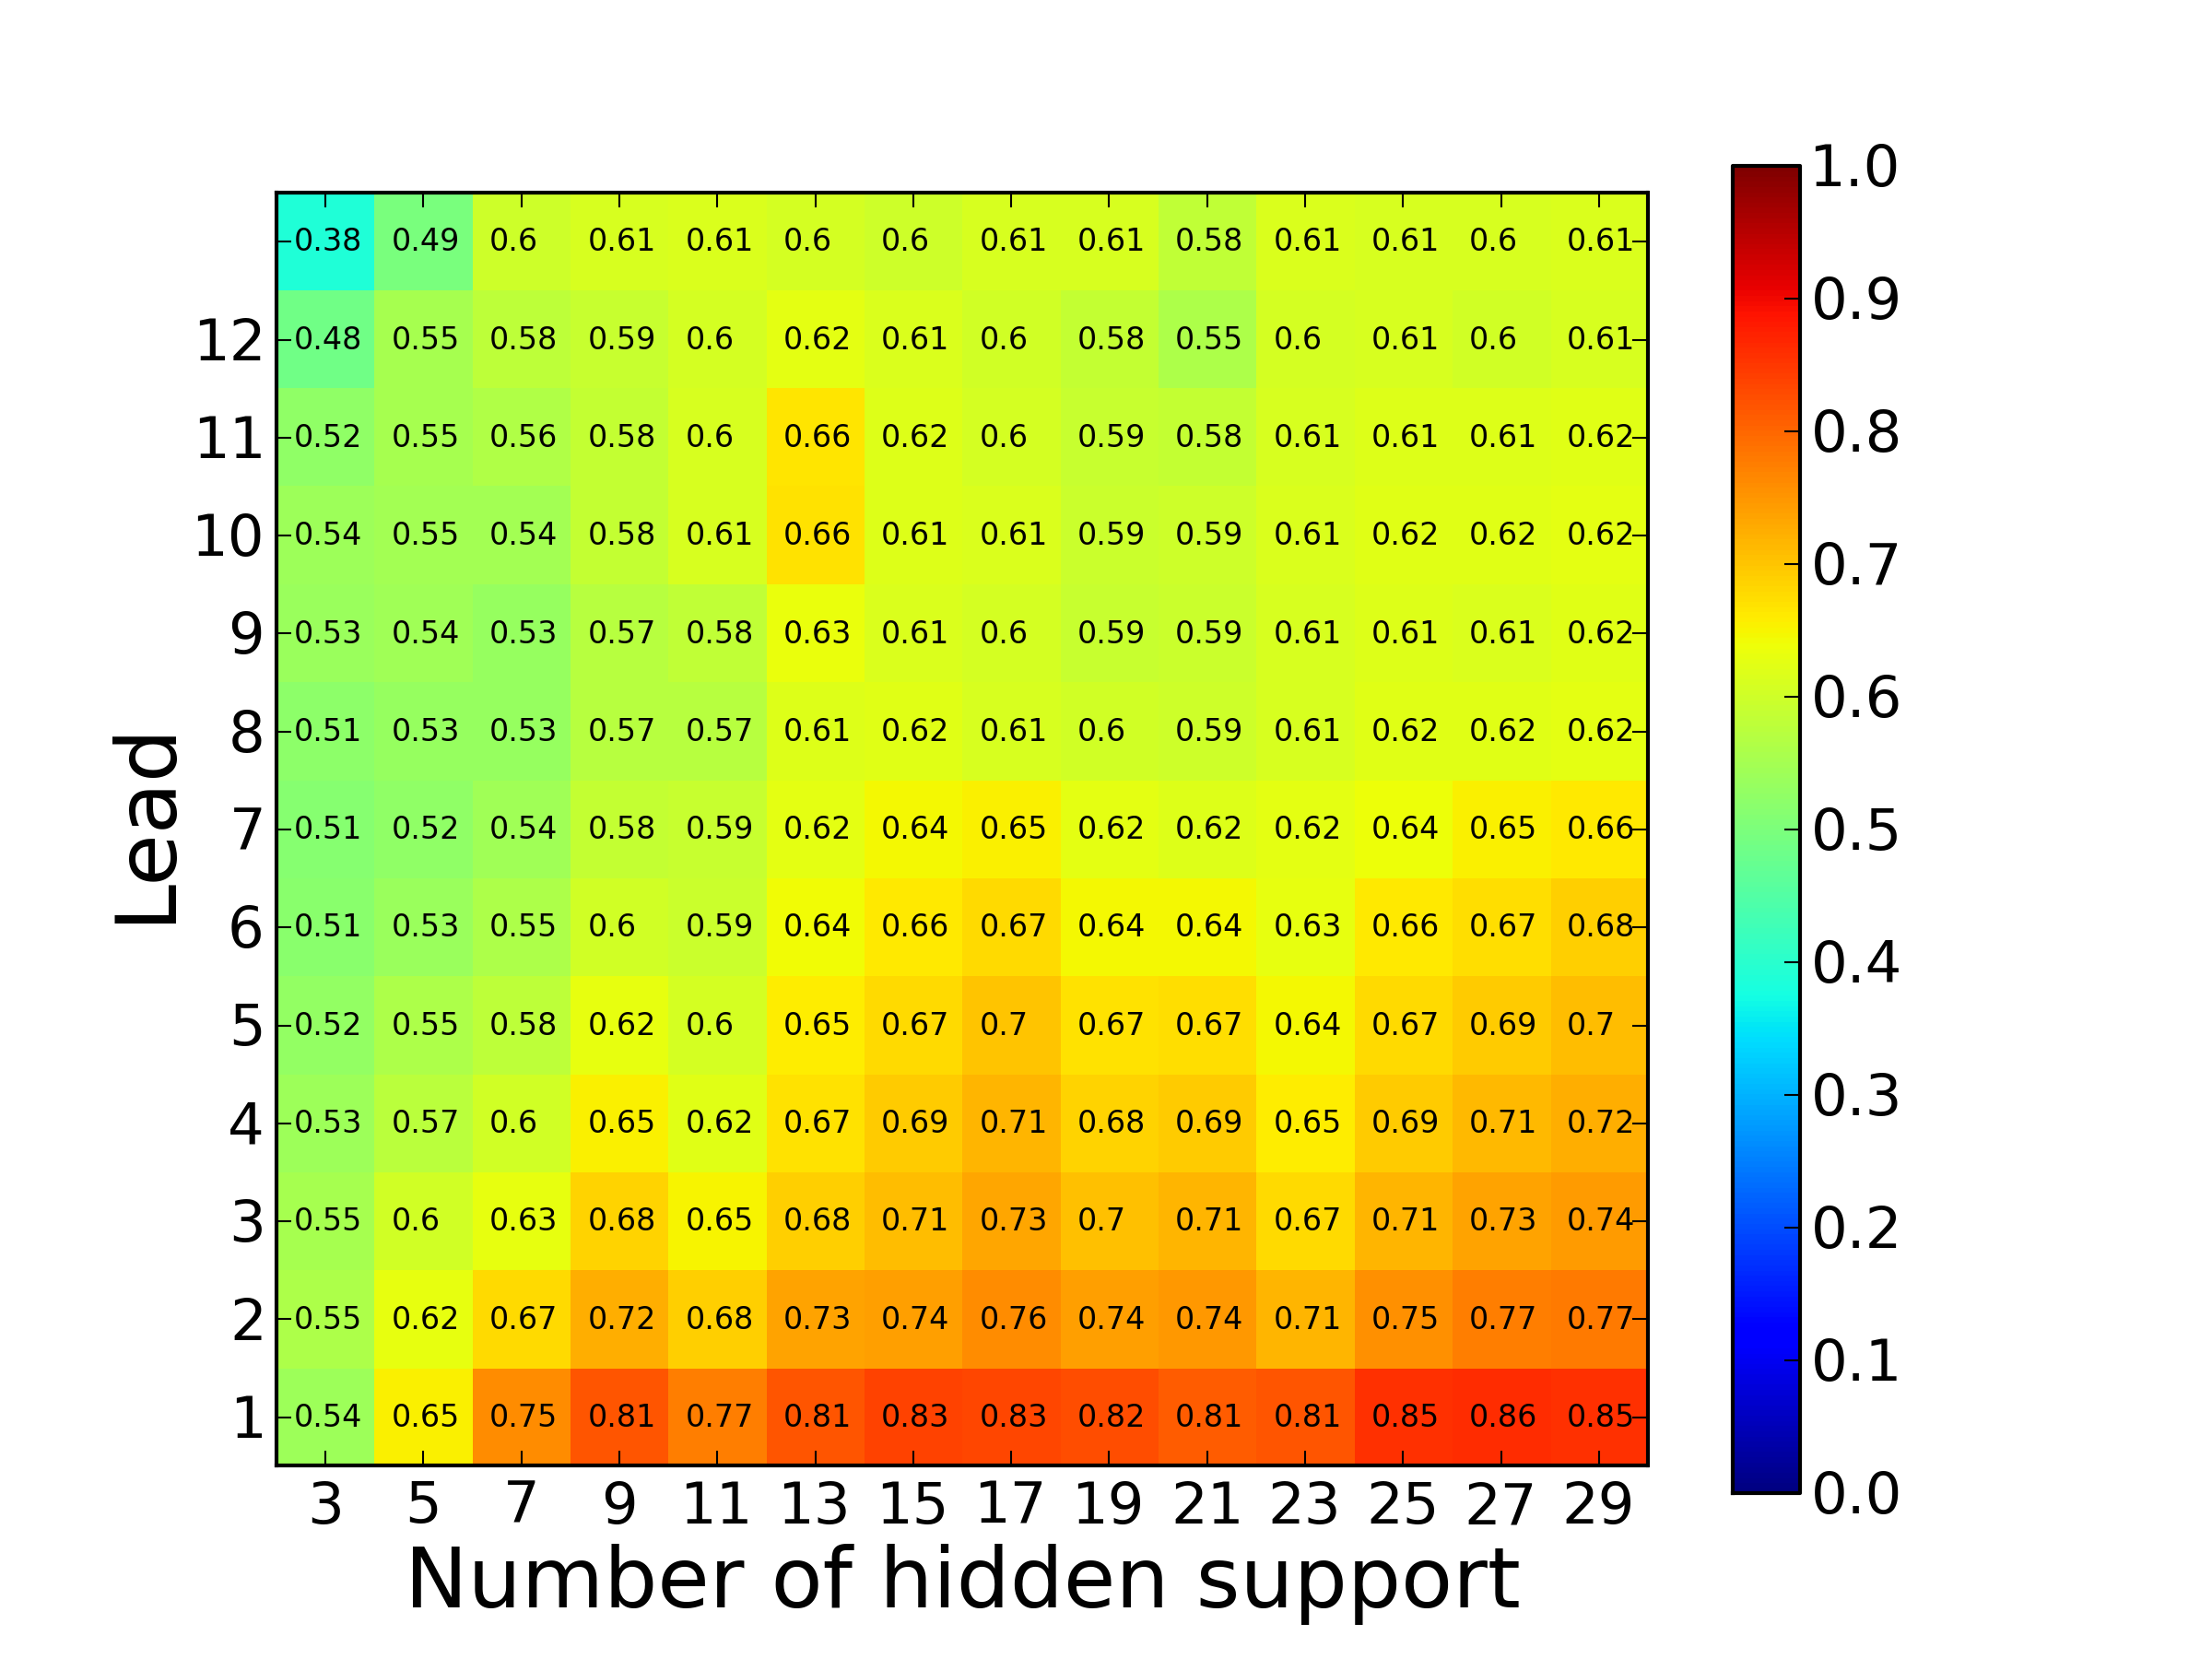
\includegraphics[width=1.0\textwidth]{figures/hmm/no_collab_pca.png}
\end{figure}

\begin{figure}[ht!]
  \caption{Heatmap for the \forum cohort. PCA transformations of features used.}\label{fig:hmm_heatmap_forum_only_pca}
  \centering
    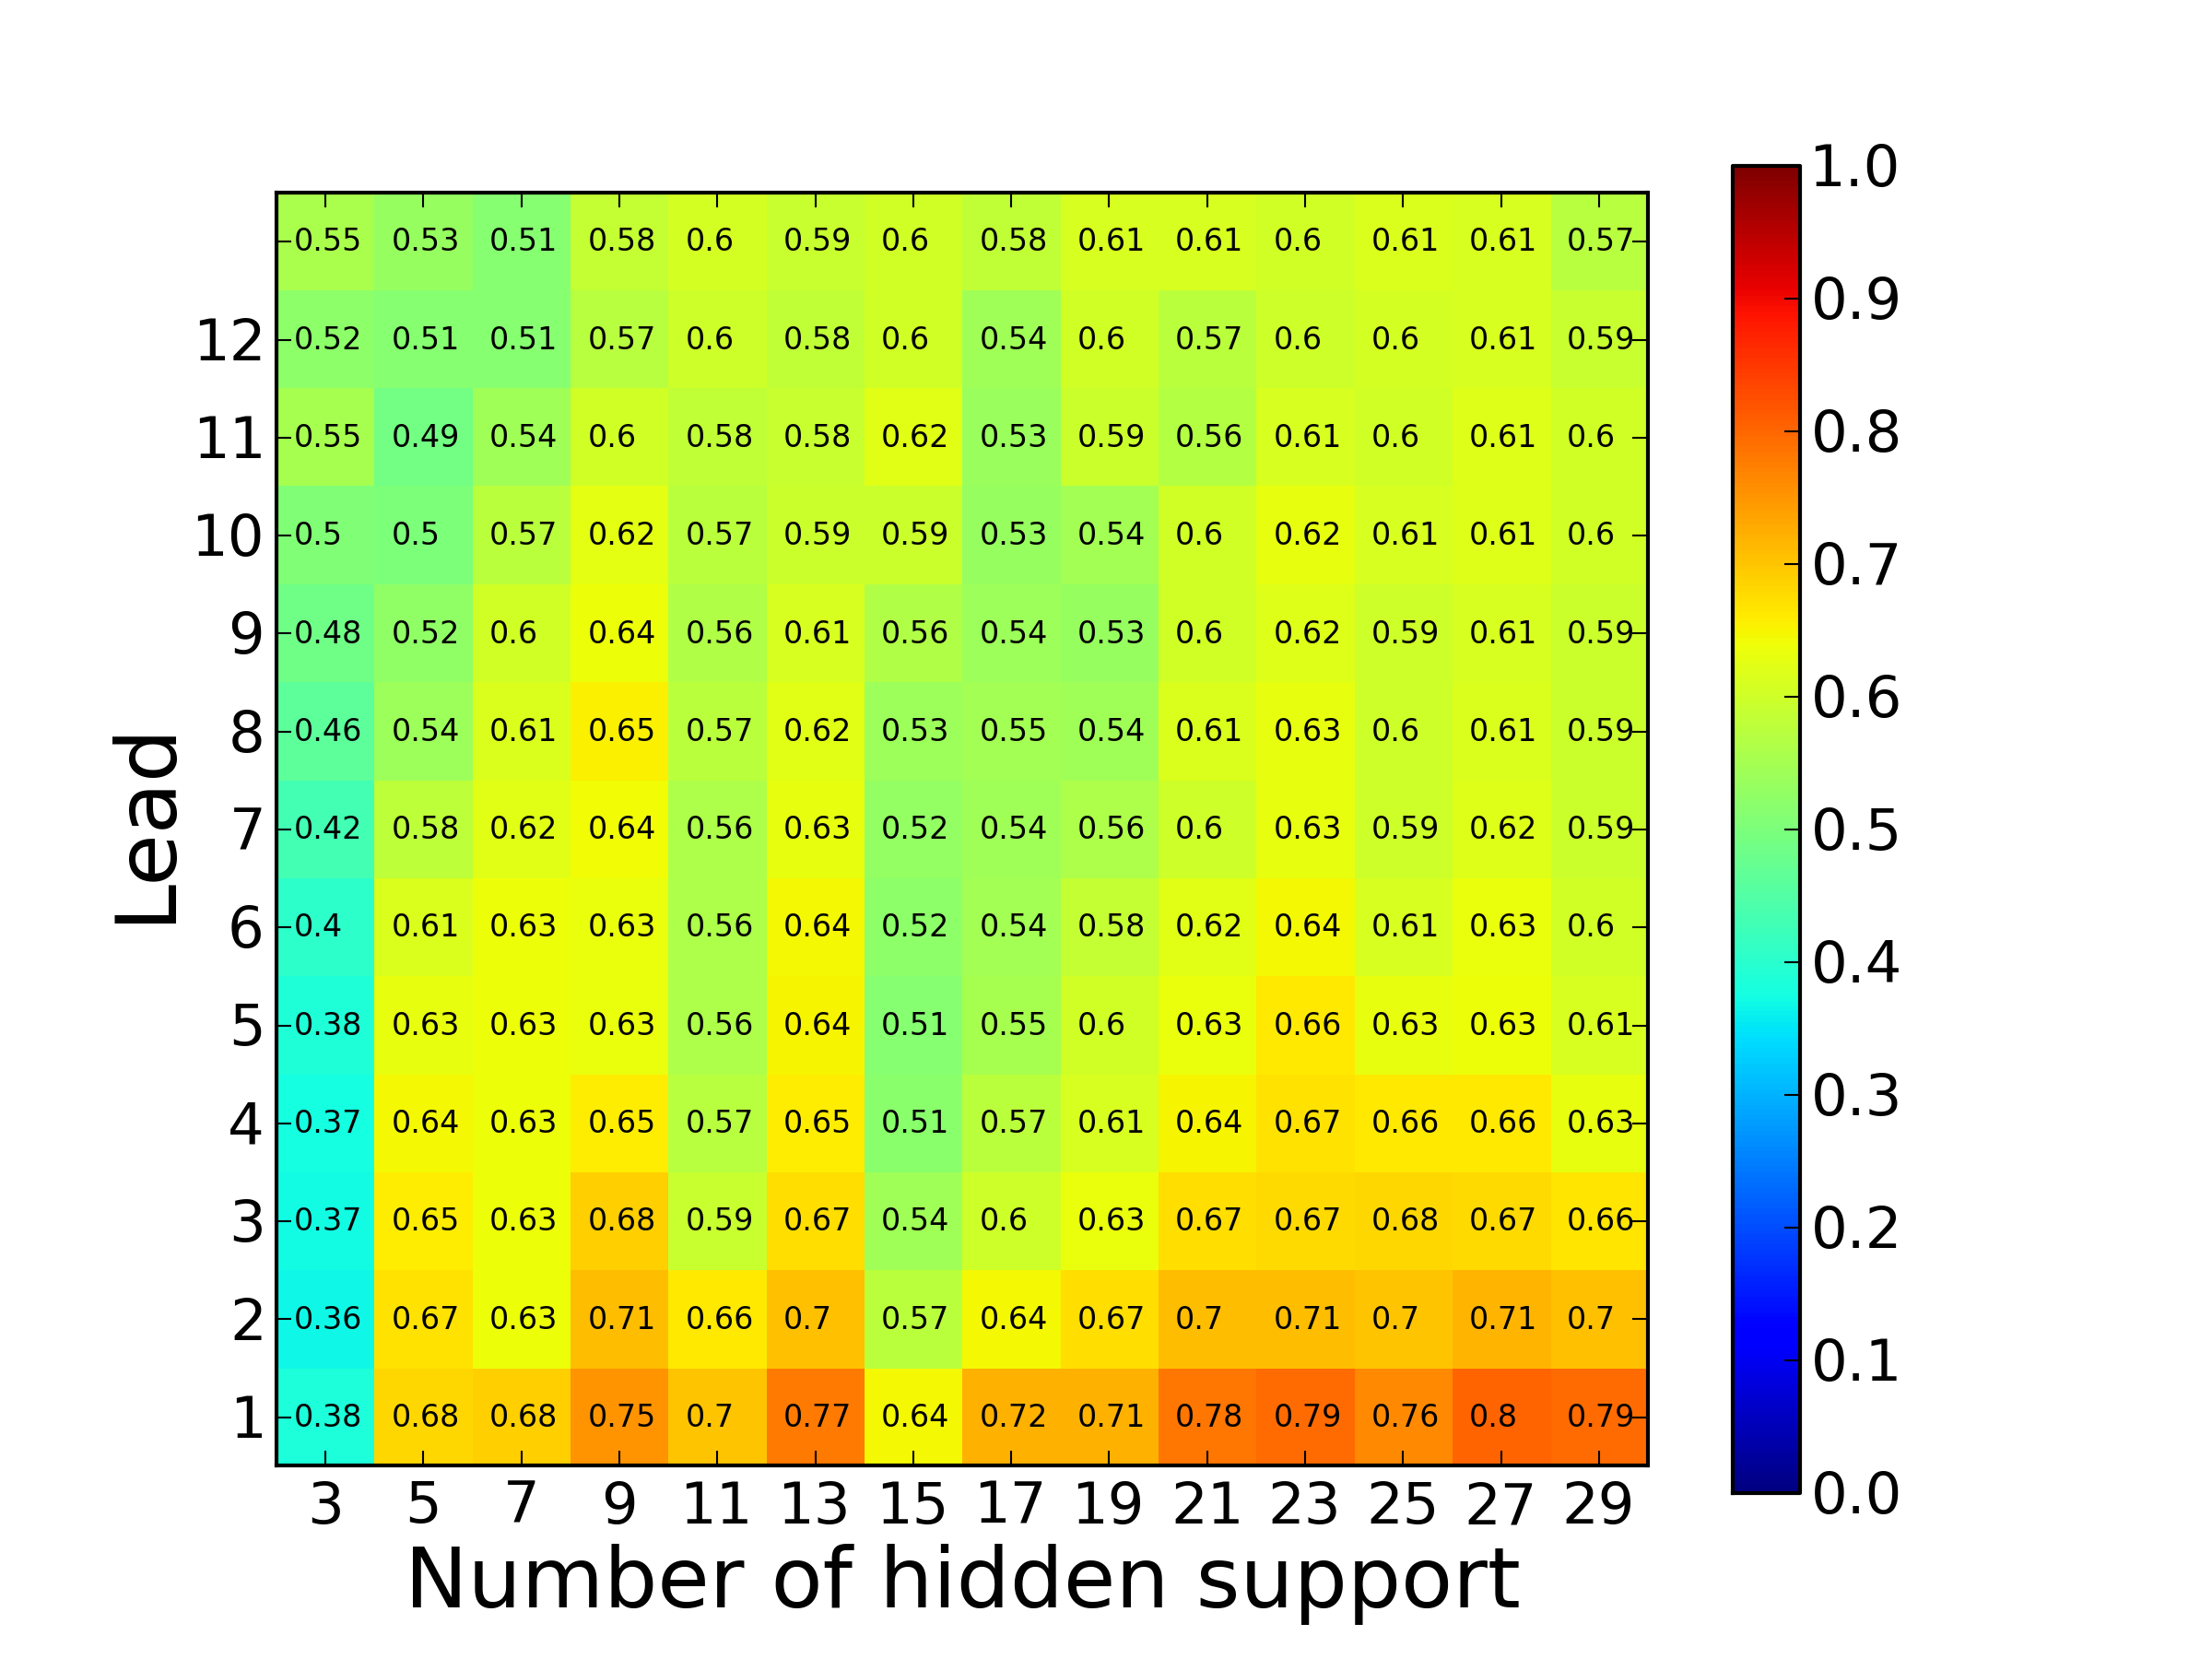
\includegraphics[width=1.0\textwidth]{figures/hmm/forum_only_pca.png}
\end{figure}

\begin{figure}[ht!]
  \caption{Heatmap for the \both cohort. PCA transformations of features used.}\label{fig:hmm_heatmap_forum_and_wiki_pca}
  \centering
    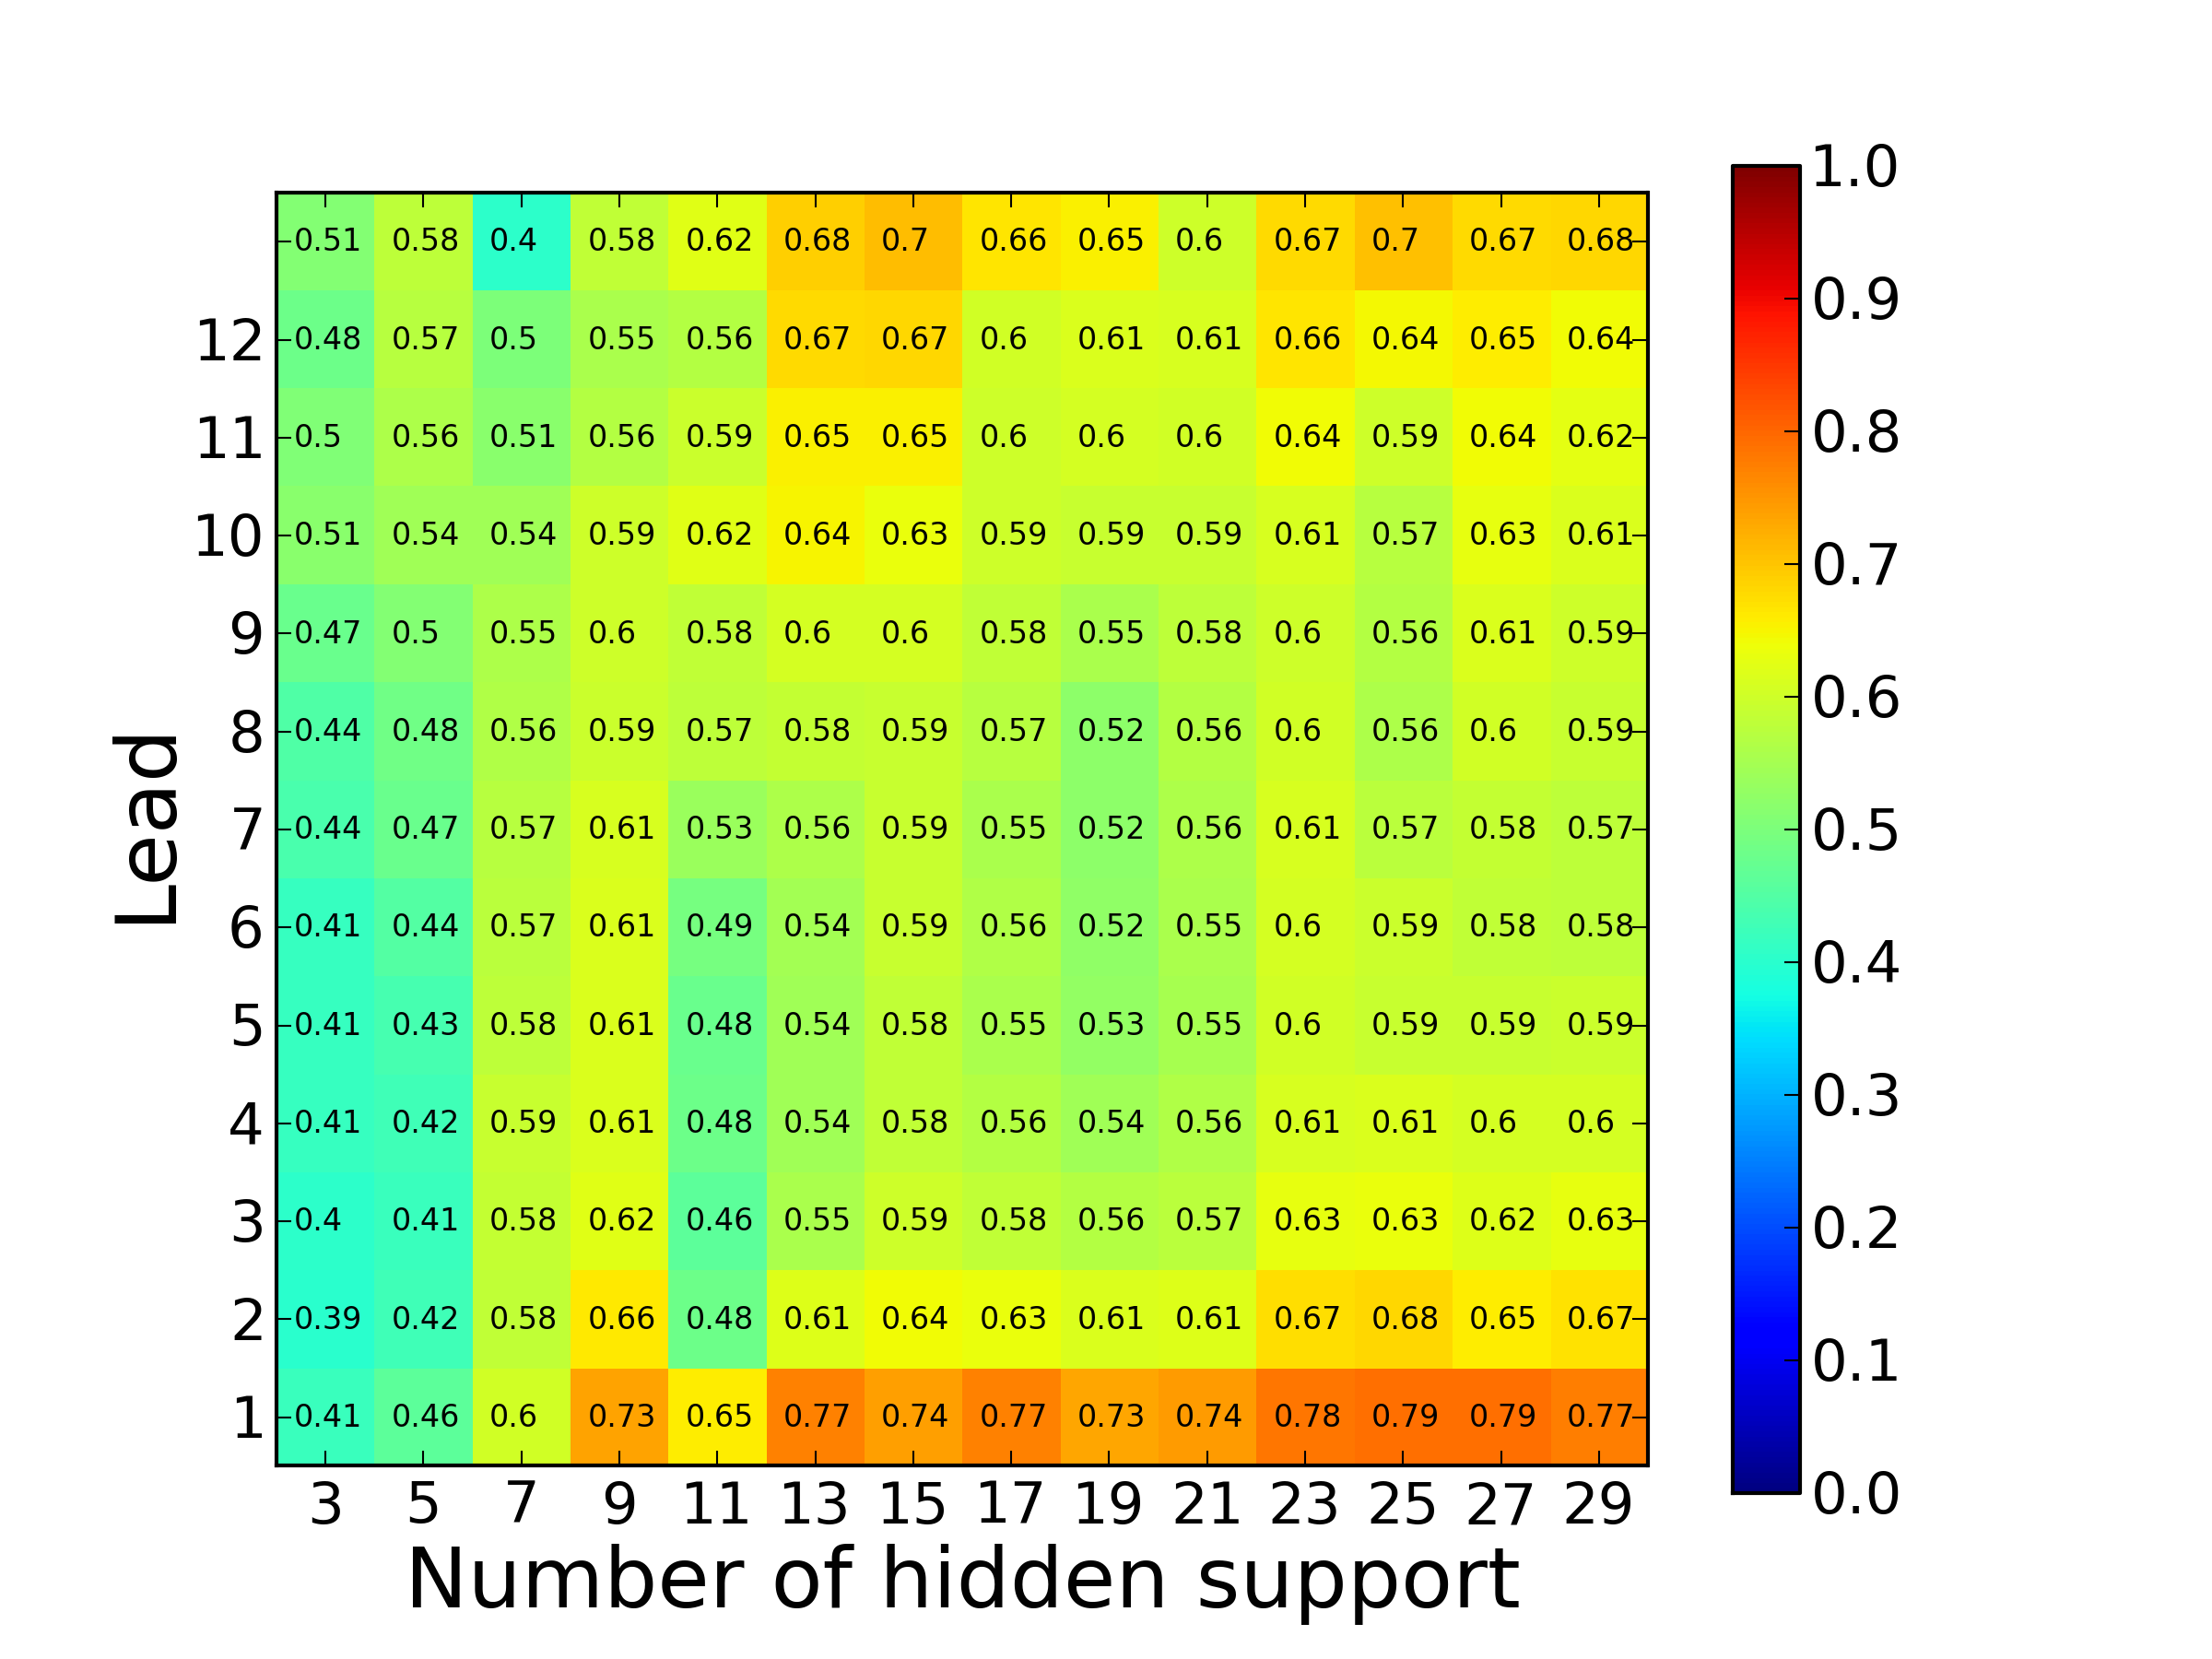
\includegraphics[width=1.0\textwidth]{figures/hmm/forum_and_wiki_pca.png}
\end{figure}

Figures \ref{fig:hmm_heatmap_no_collab_pca} to \ref{fig:hmm_heatmap_forum_and_wiki_pca} show HMM heatmaps for cohorts \neither, \forum and \both. These featuresets used PCA to reduce their dimensionality. We were unable to use PCA to reduce the \wiki cohort because it was too small. Each heatmap visualizes the ROC AUC for various leads as we vary K to create different models.

The PCA HMM models require a relatively larger K value in order to converge to a high AUC. For the \neither cohort, for example, we see that increasing K continually increases AUCs for all leads, up through a K of 29. This suggests that there are even more than 29 modes of students, and that we could attain even better results through a higher K value. The PCA HMMs show a large contrast between high leads and low leads. However, as compared with logistic regression, we see more consistent results cross the cohorts. For example, with a lead of one, the \neither, \forum and \both cohorts are within 0.08 of each other. In logistic regression, there is a difference in AUC of 0.2.

We suspect that the high difference in predictive accuracies between high leads and low leads is due to the fact that HMMs use a single transition matrix for all weeks. There is likely to be different probabilities of transferring hidden state between weeks 1 and 2 than between 12 and 13, for example, but the HMM posits only one set of probabilities. Furthermore, since there are more students in earlier weeks due to stopout, the transition matrix will have more examples from earlier weeks. Thus, it will be biased towards the earlier weeks, allowing for better prediction in the earlier weeks than in later weeks. 

\begin{figure}[ht!]
  \caption{Mean AUC as K increases for the \neither cohort. PCA transformations of features used.}\label{fig:hmm_support_over_time_no_collab_pca}
  \centering
    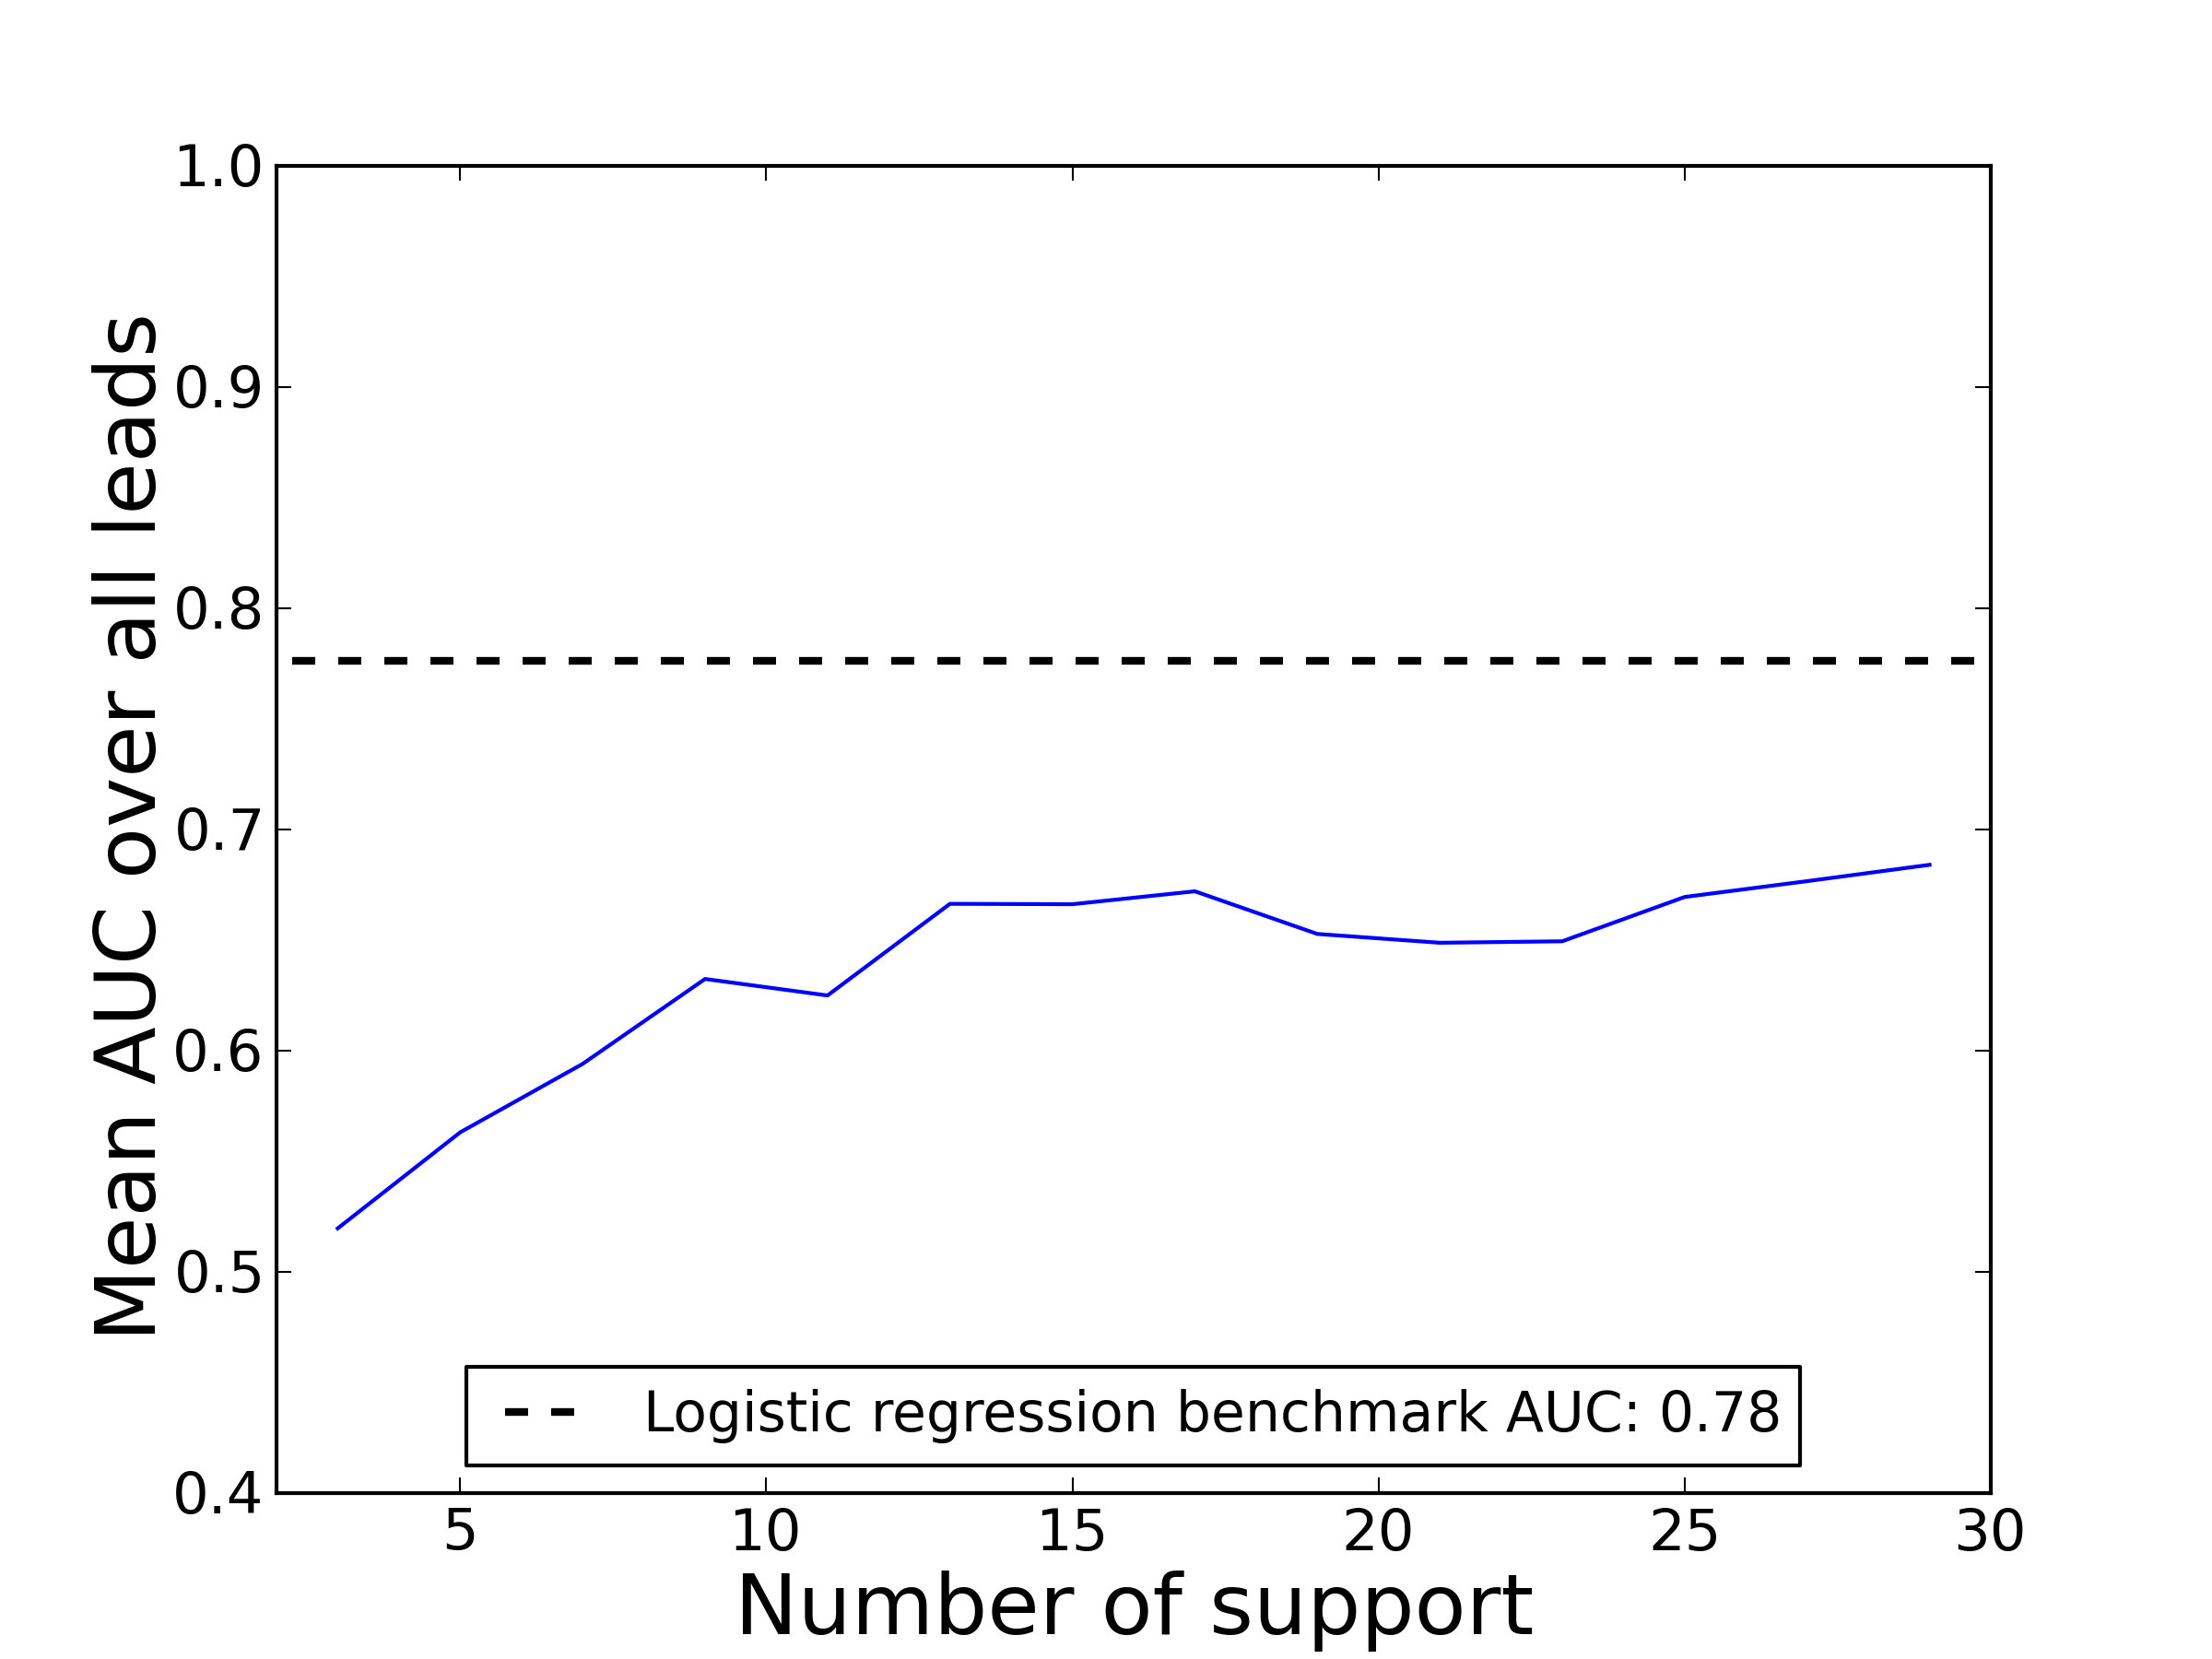
\includegraphics[width=0.8\textwidth]{figures/hmm/no_collab_pca_support_over_time.png}
\end{figure}

\begin{figure}[ht!]
  \caption{Mean AUC as K increases for the \forum cohort. PCA transformations of features used.}\label{fig:hmm_support_over_time_forum_only_pca}
  \centering
    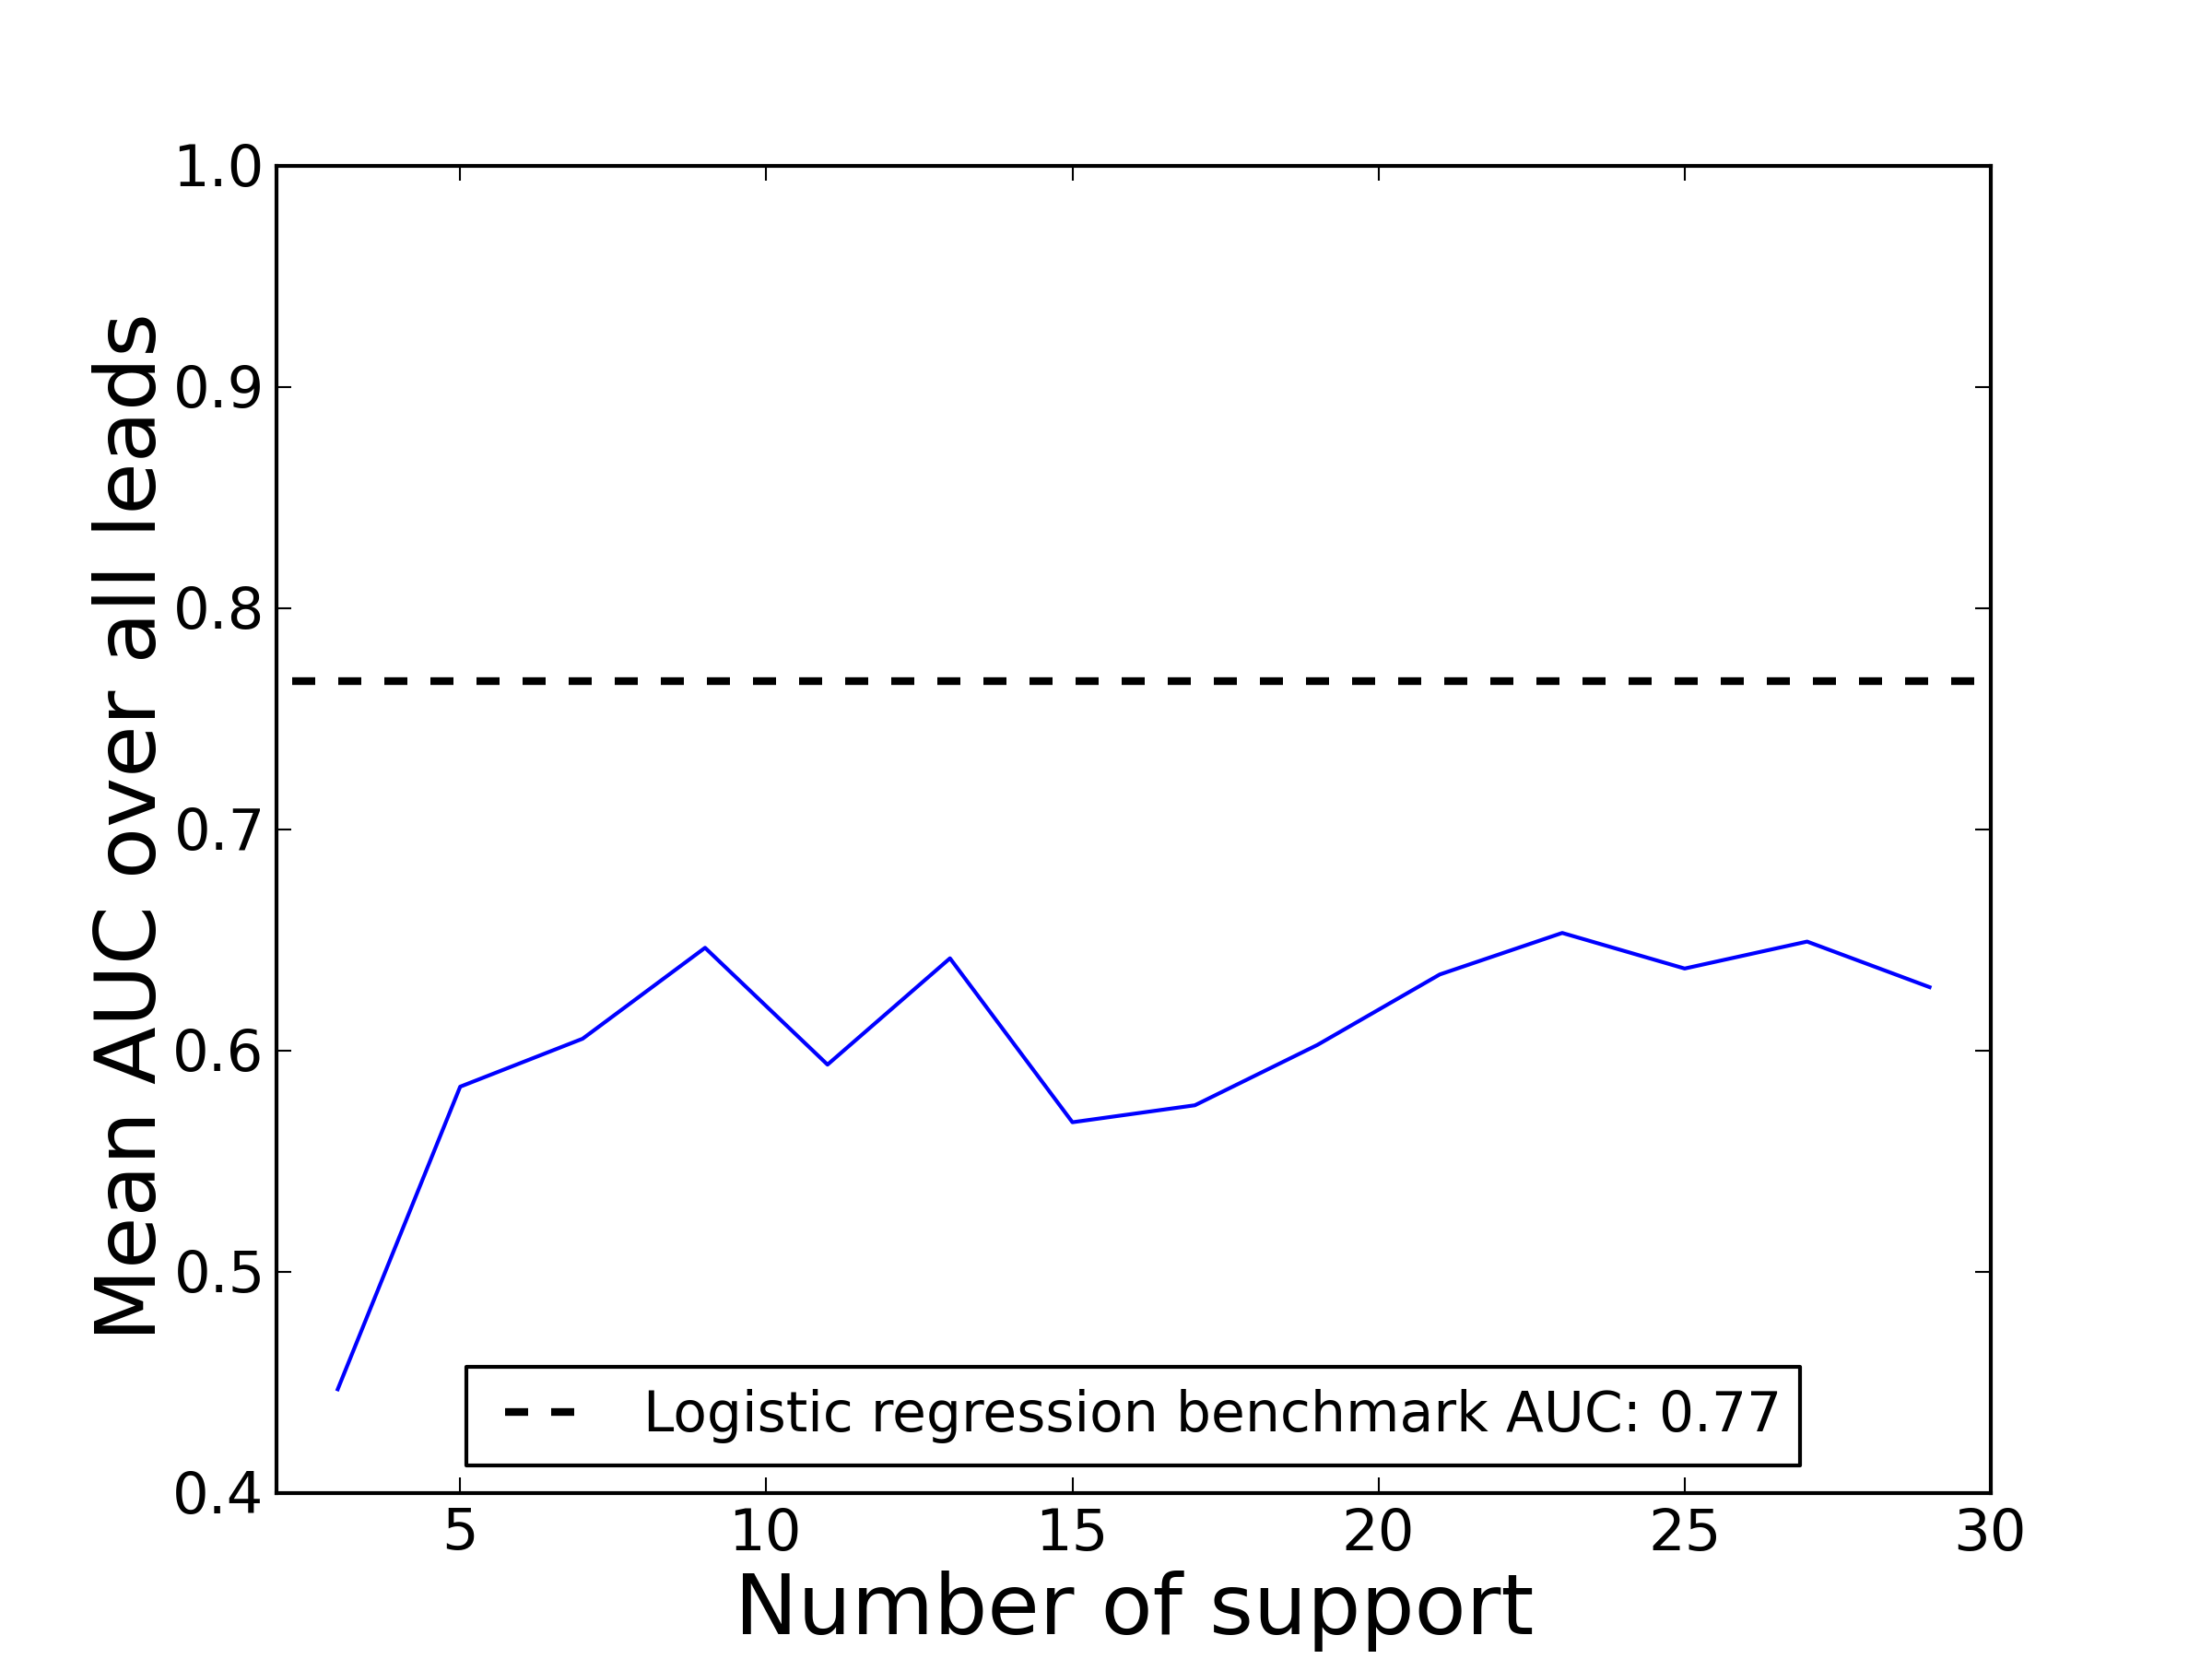
\includegraphics[width=0.8\textwidth]{figures/hmm/forum_only_pca_support_over_time.png}
\end{figure}

\begin{figure}[ht!]
  \caption{Mean AUC as K increases for the \both cohort. PCA transformations of features used.}\label{fig:hmm_support_over_time_forum_and_wiki_pca}
  \centering
    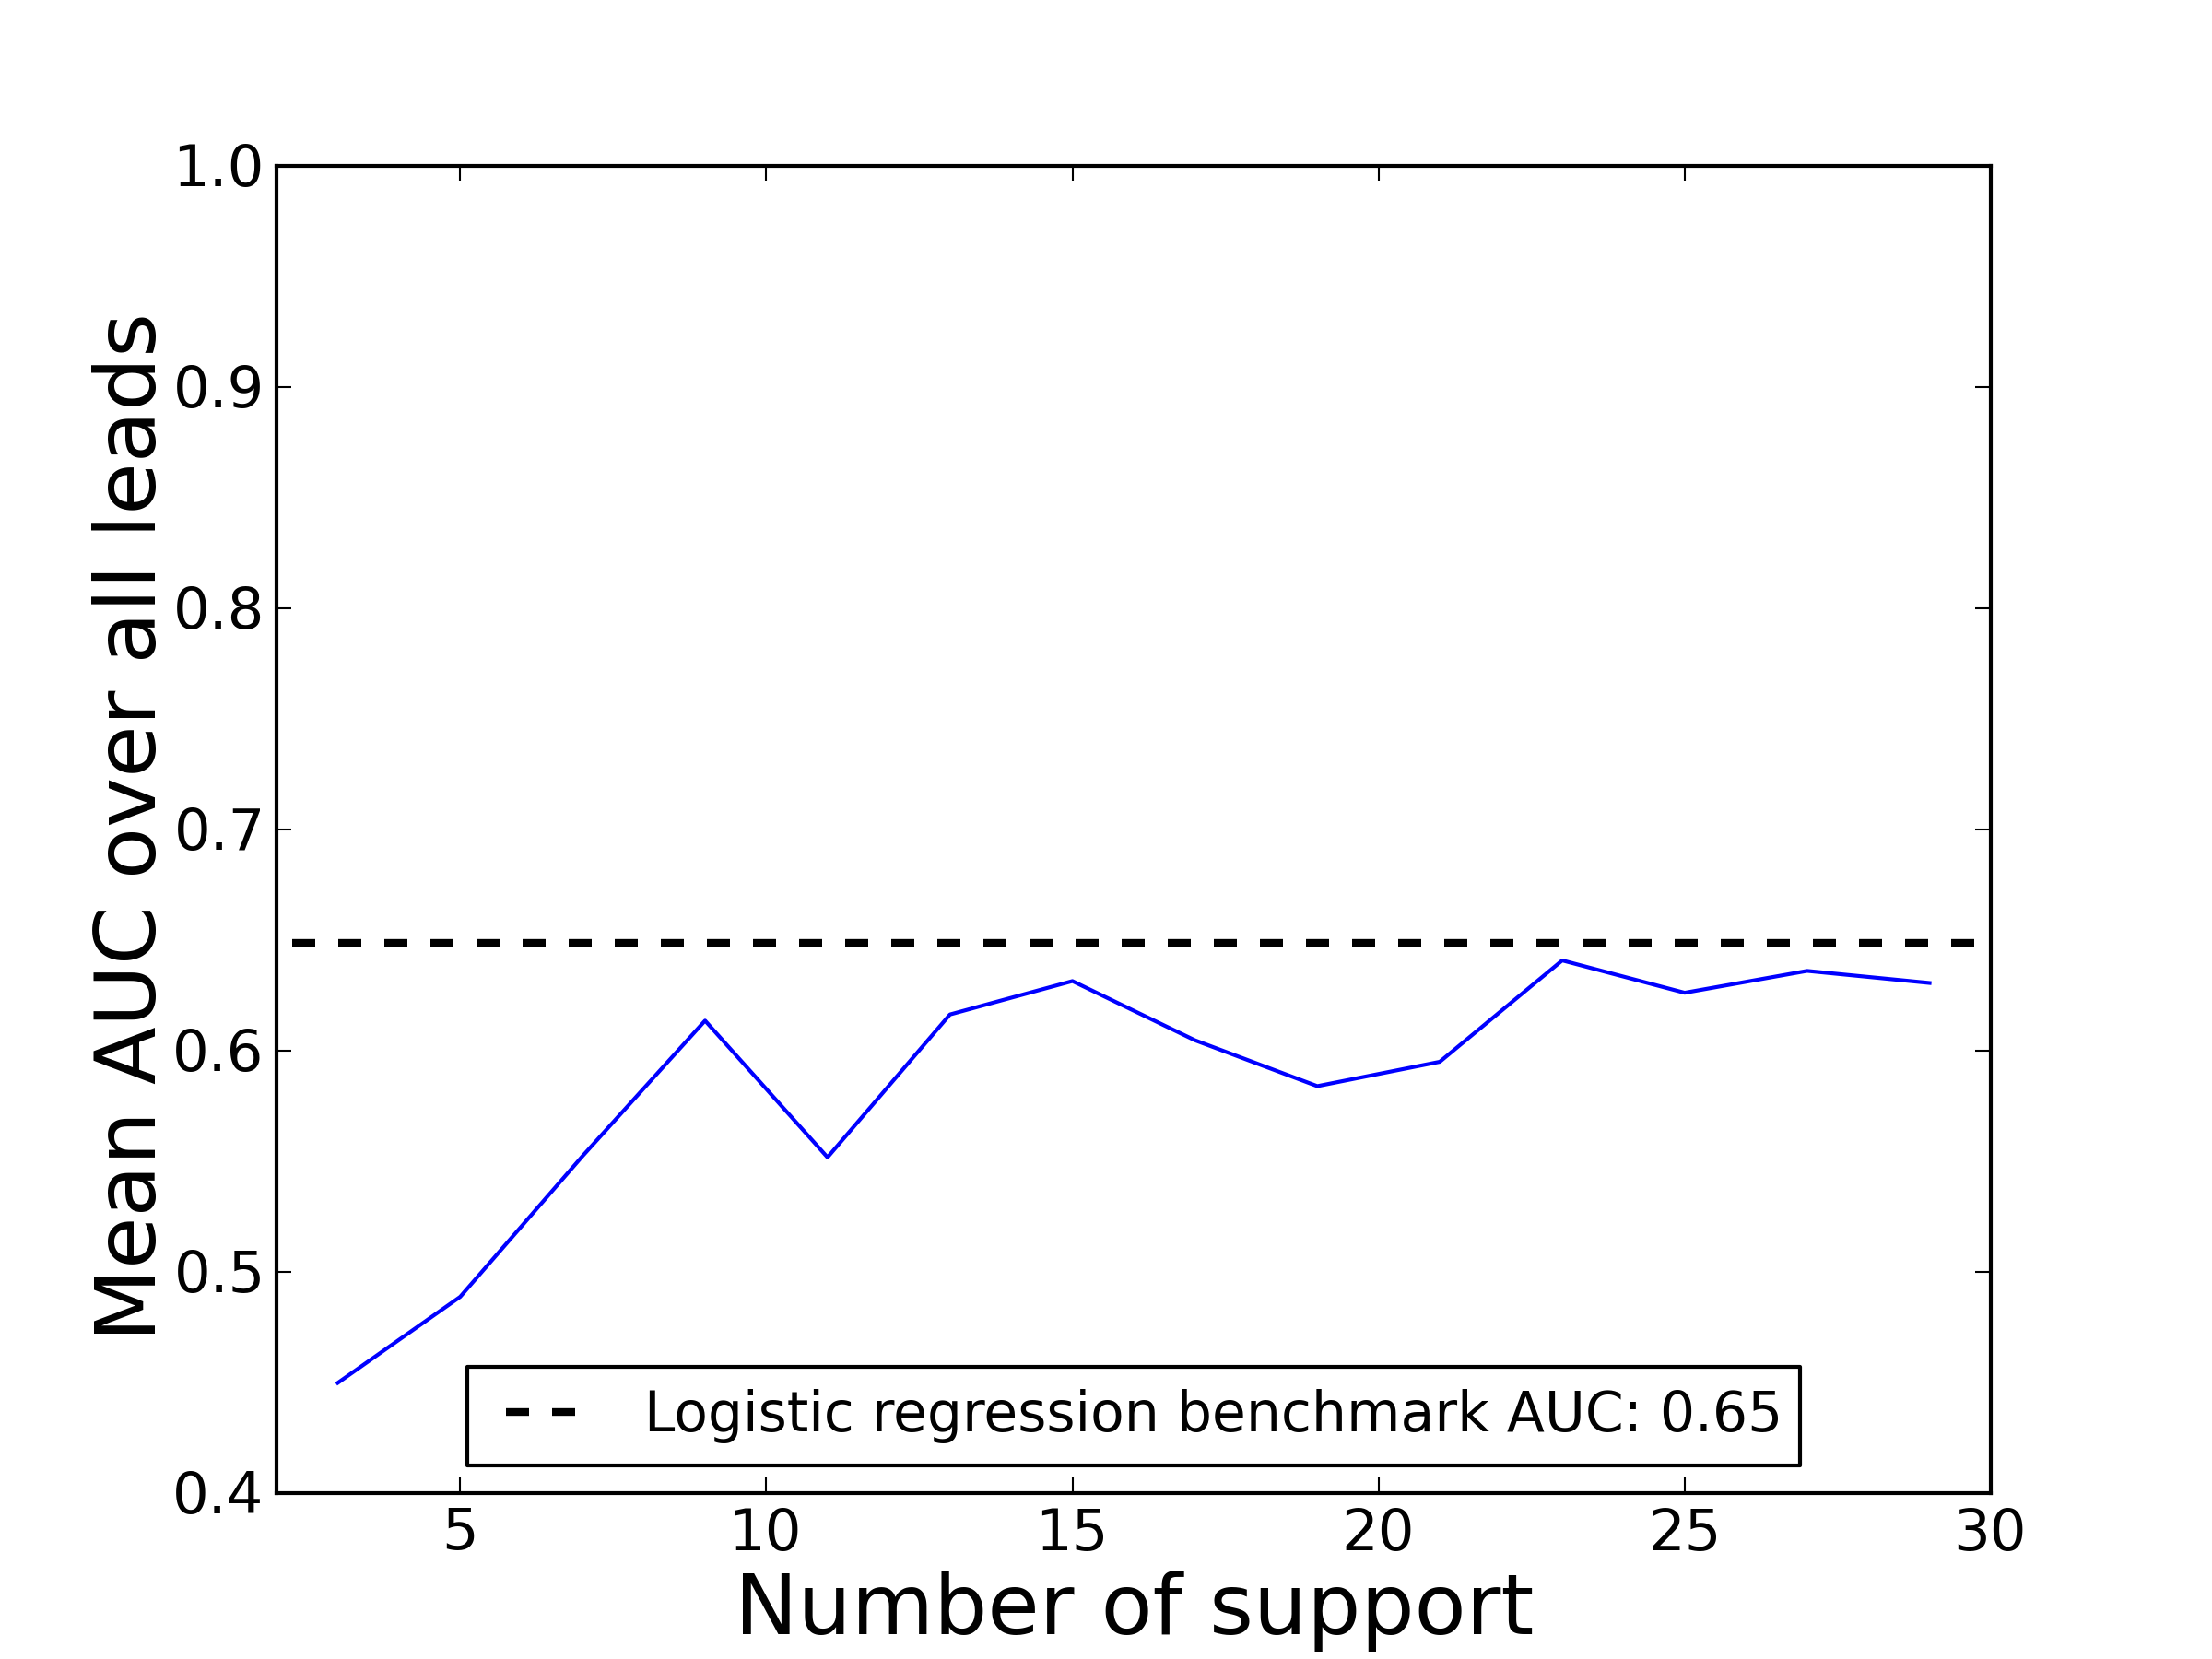
\includegraphics[width=0.8\textwidth]{figures/hmm/forum_and_wiki_pca_support_over_time.png}
\end{figure}


The following line graphs show how overall predictive accuracies of the PCA HMM models change as K increases. These graphs indicate the correct number of hidden states needed in order to model each cohort. See Figures \ref{fig:hmm_support_over_time_no_collab_pca} through 
\ref{fig:hmm_support_over_time_forum_and_wiki_pca}. The mean prediction AUC of all 91 experiments for logistic regression is also shown for each cohort as a benchmark.

The results again indicate that the \forum and \both cohorts seem to have converged, but not until K has reached ~25. However, the \neither cohort's mean AUC is still increasing as K goes to 29, indicating that a higher K could better model this cohort.

\begin{figure}[ht!]
  \caption{Heatmap for the \neither cohort.}\label{fig:hmm_heatmap_no_collab}
  \centering
    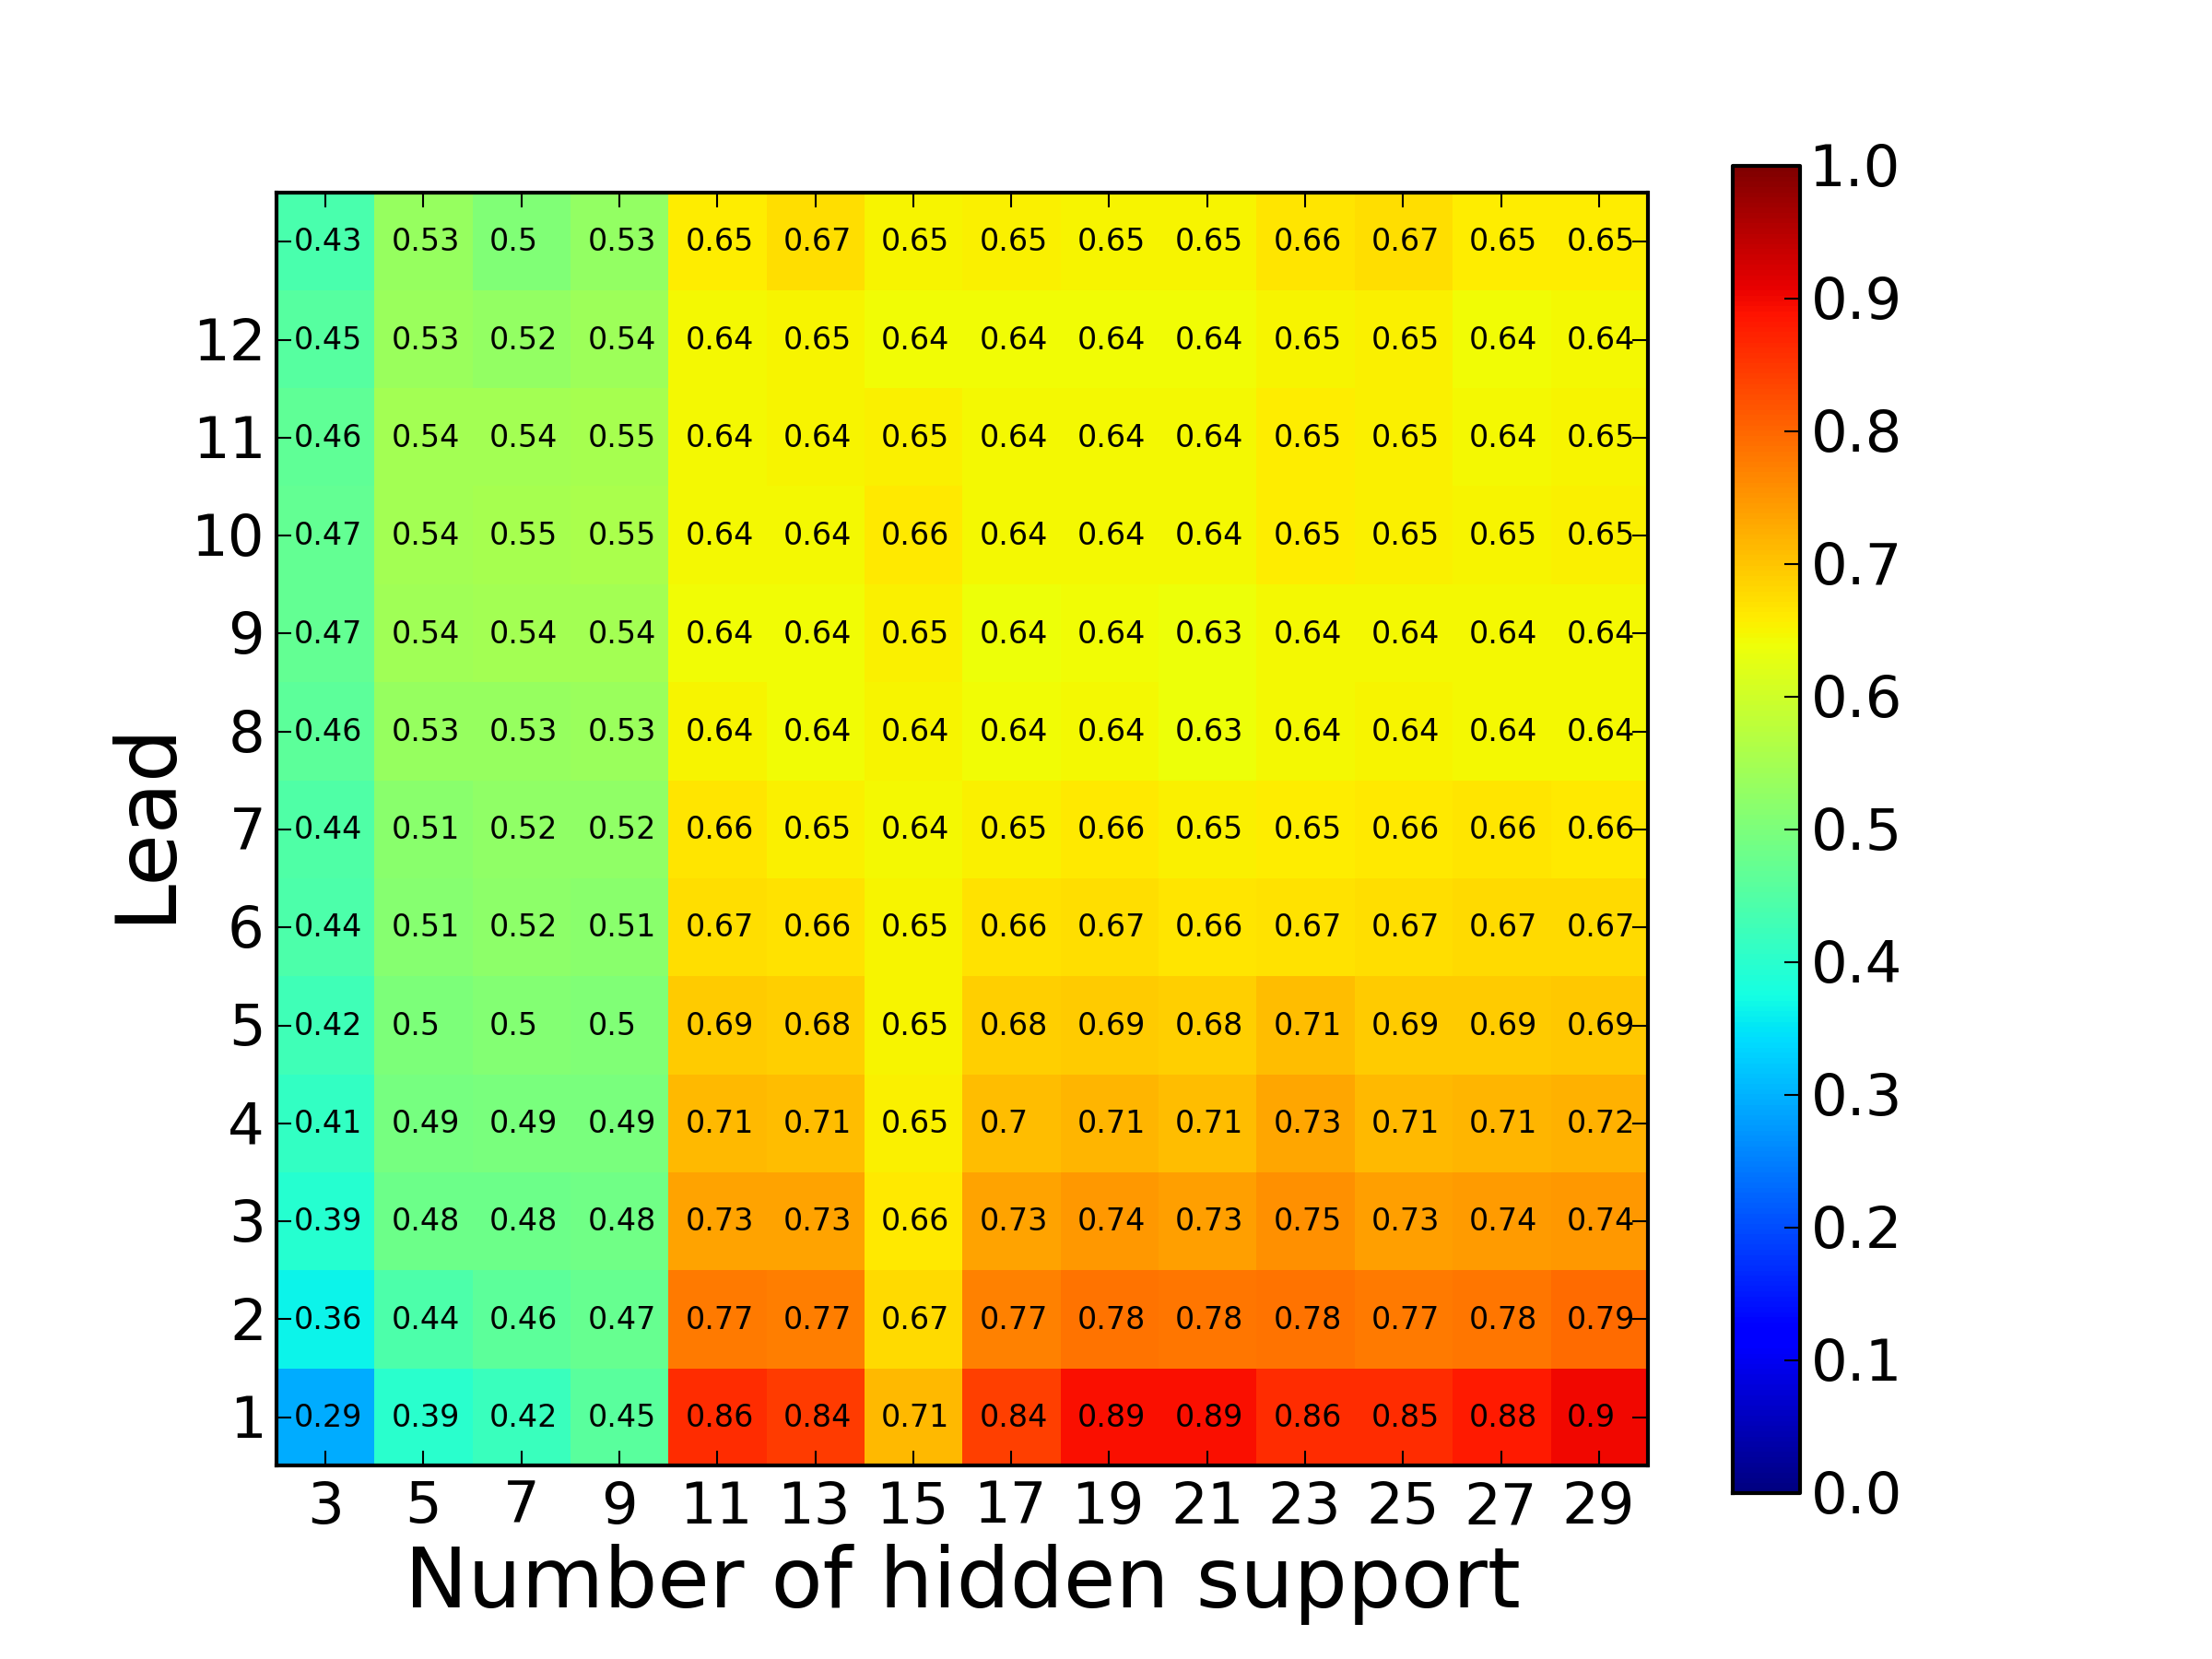
\includegraphics[width=1.0\textwidth]{figures/hmm/no_collab.png}
\end{figure}

\begin{figure}[ht!]
  \caption{Heatmap for the \forum cohort.}\label{fig:hmm_heatmap_forum_only}
  \centering
    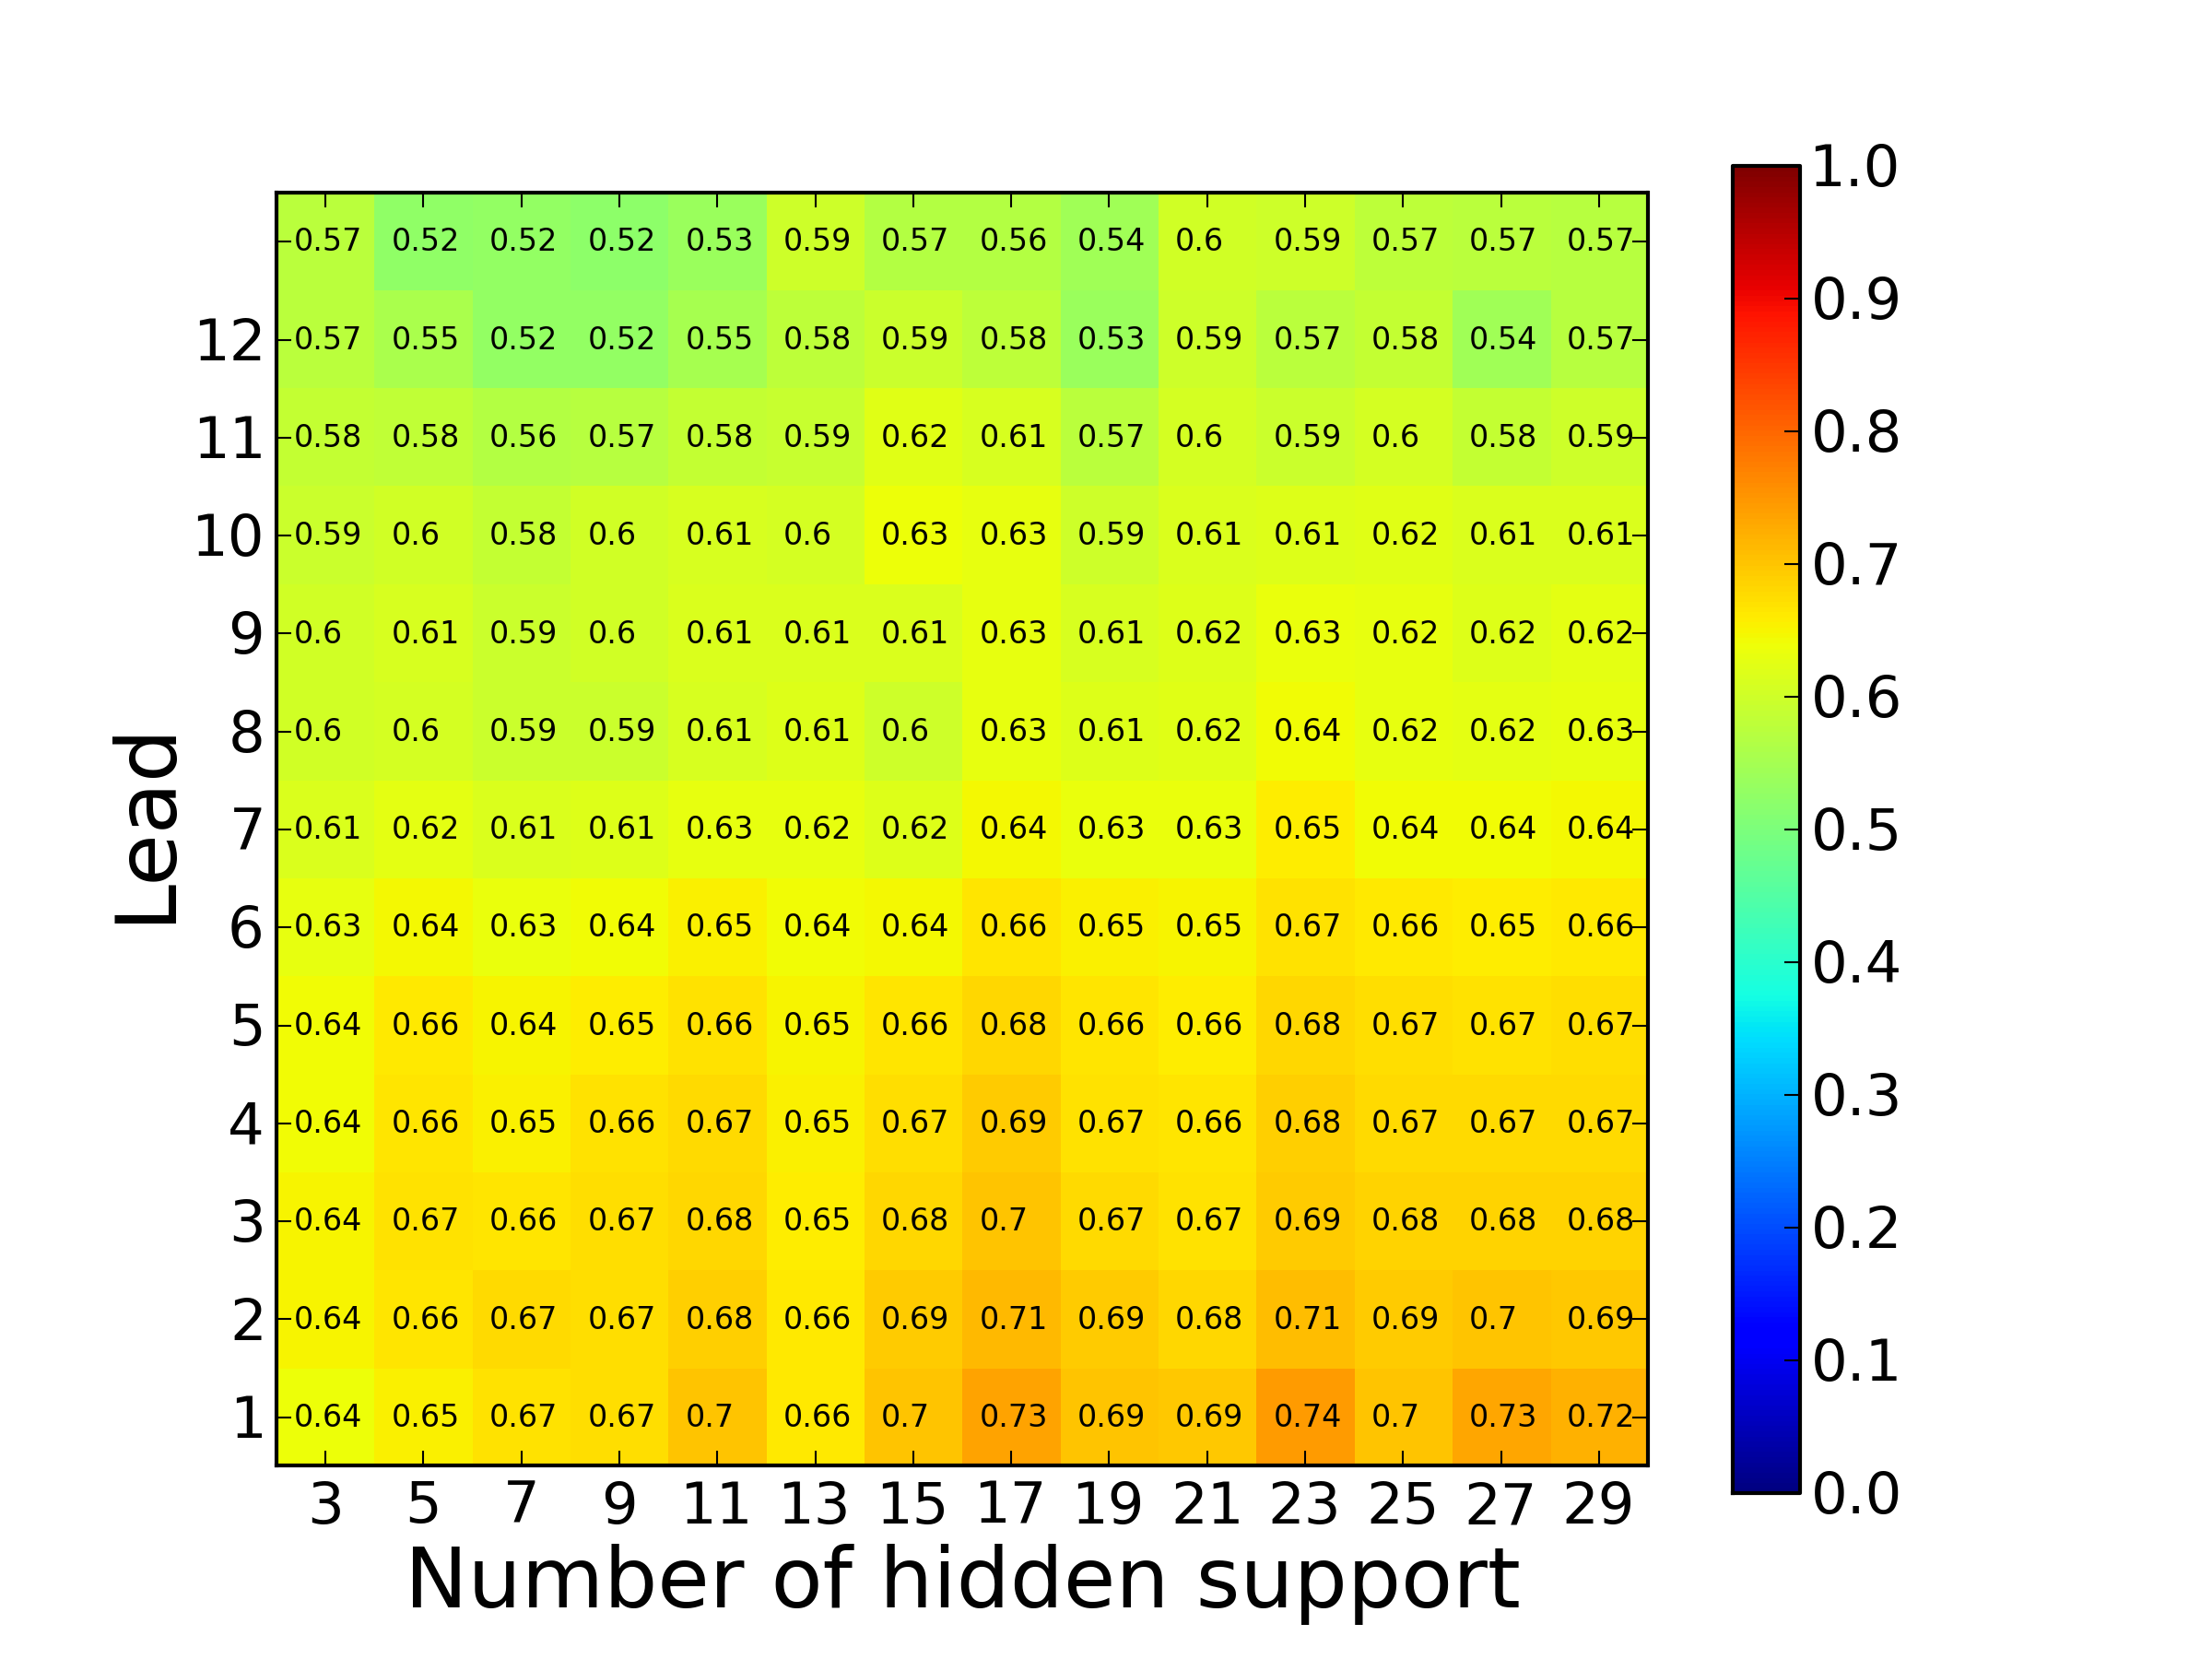
\includegraphics[width=1.0\textwidth]{figures/hmm/forum_only.png}
\end{figure}

\begin{figure}[ht!]
  \caption{Heatmap for the \both cohort.}\label{fig:hmm_heatmap_forum_and_wiki}
  \centering
    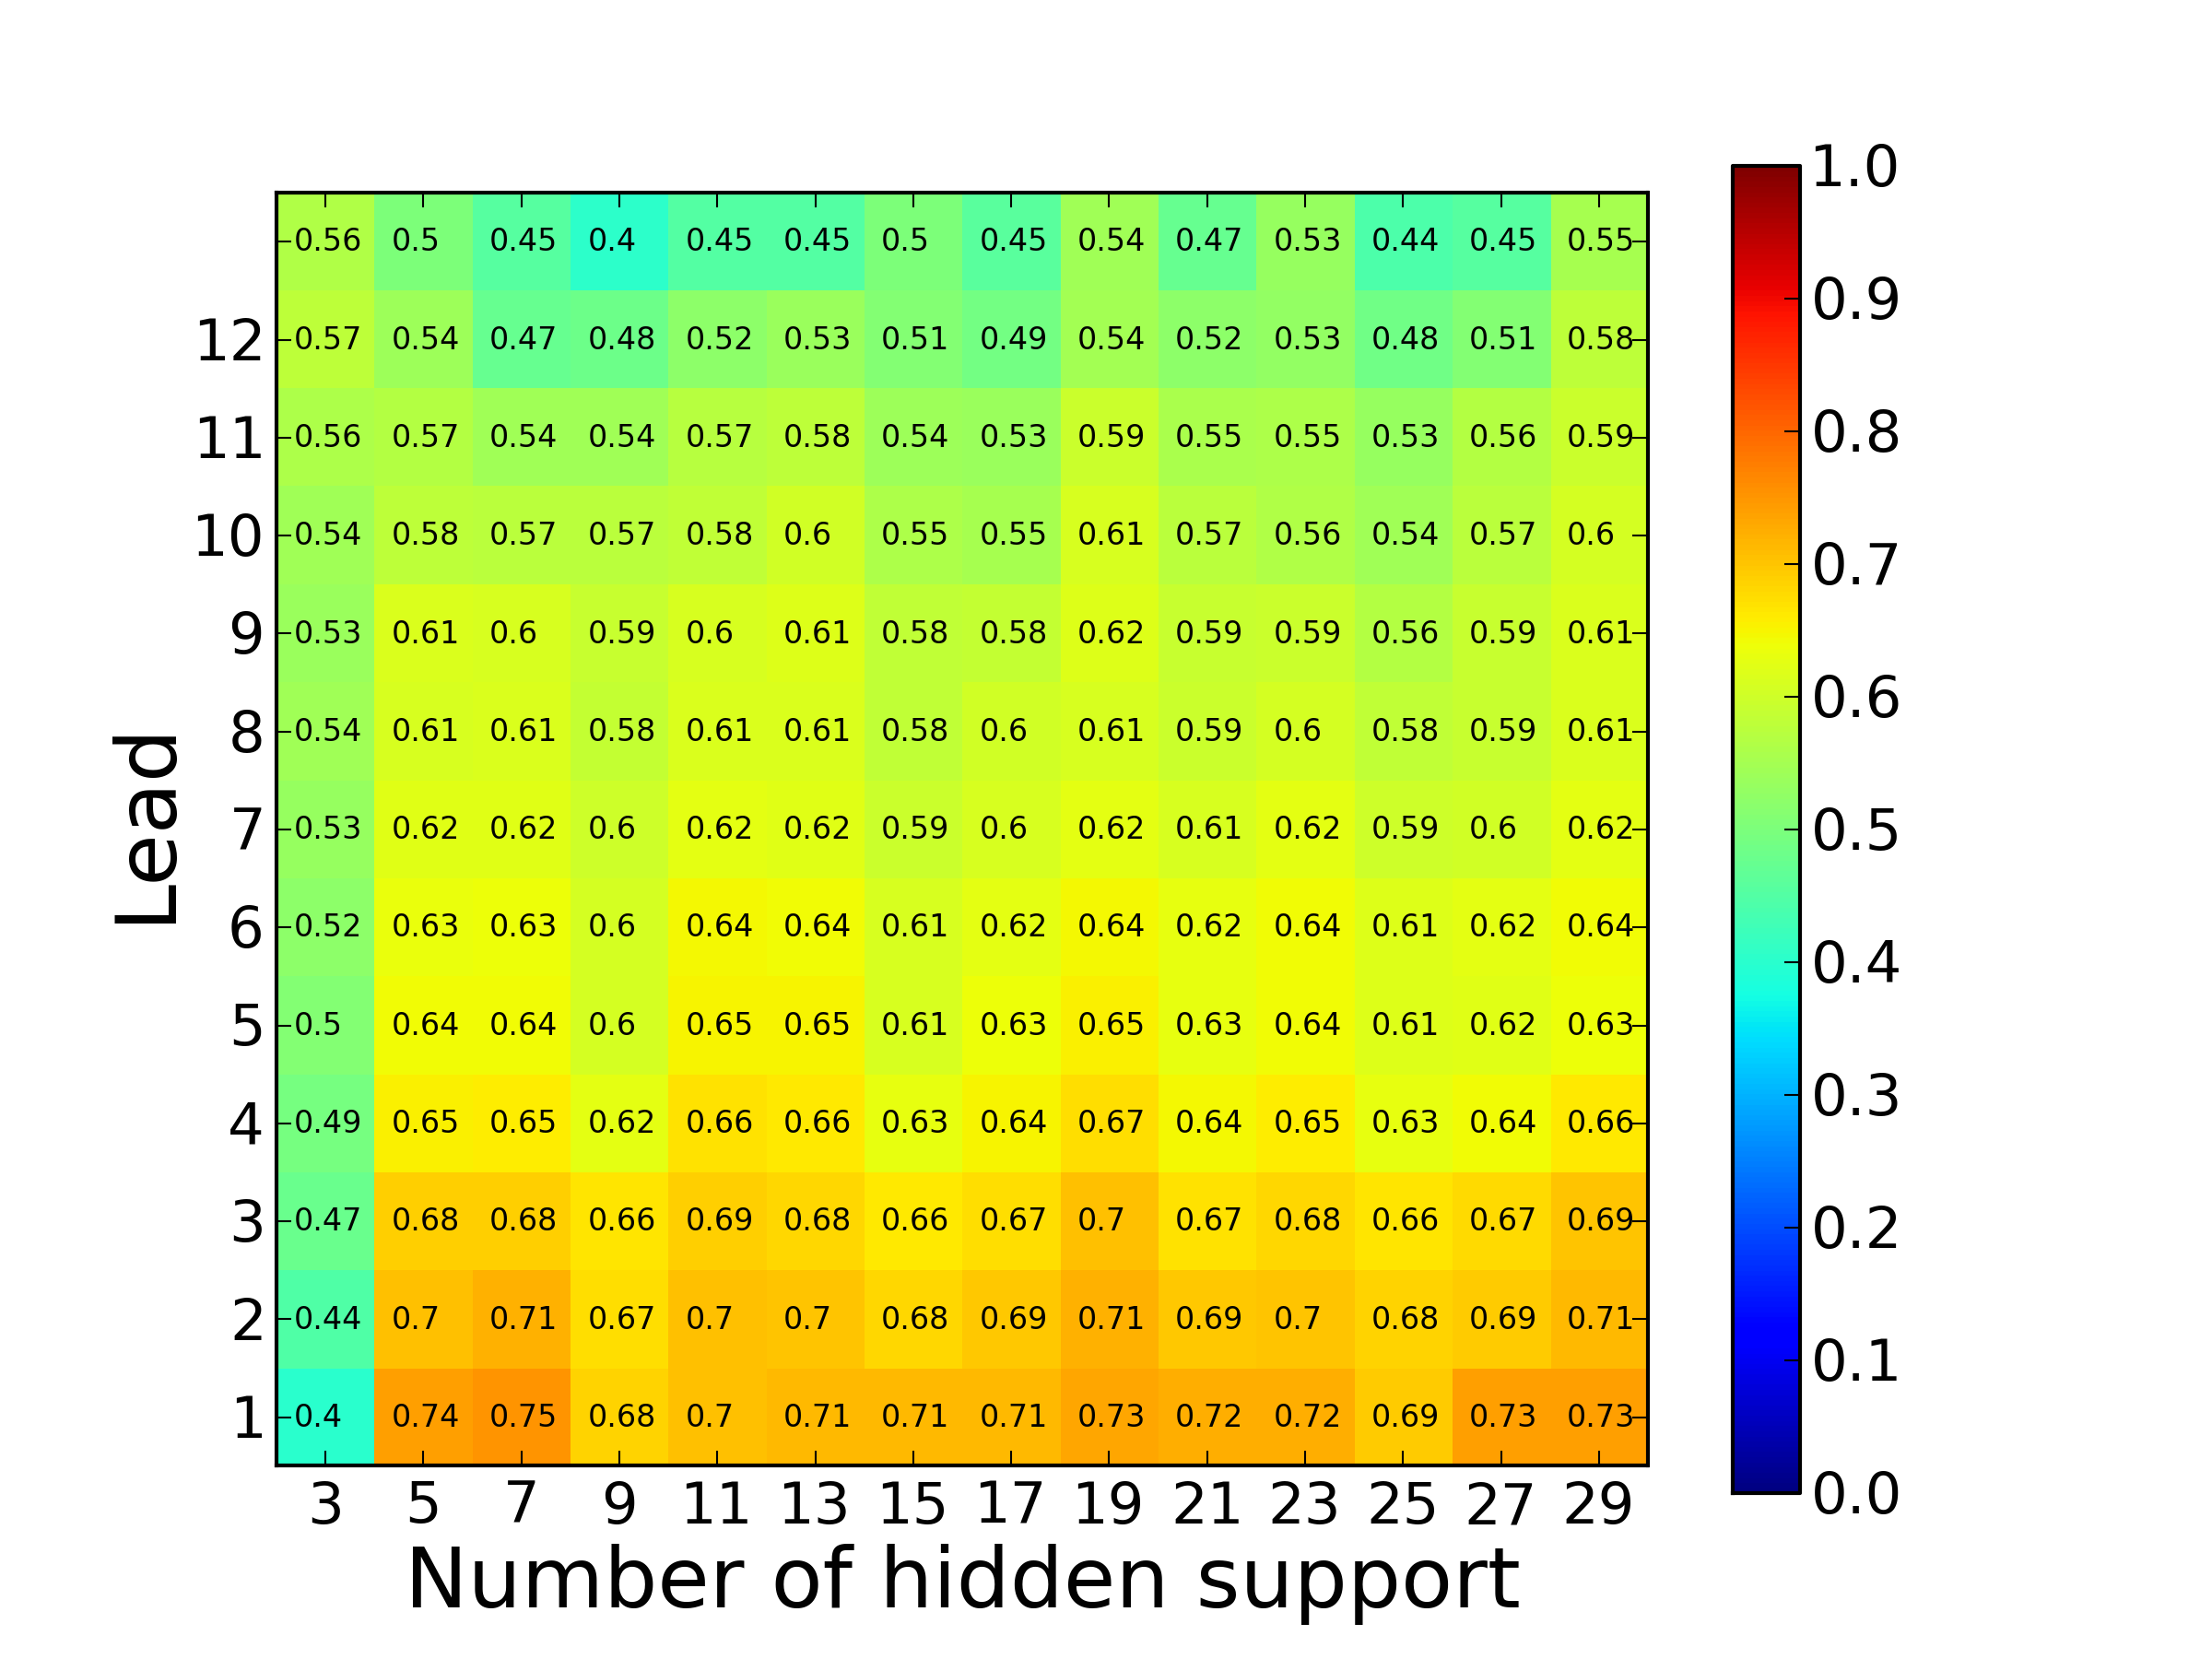
\includegraphics[width=1.0\textwidth]{figures/hmm/forum_and_wiki.png}
\end{figure}

\begin{figure}[ht!]
  \caption{Heatmap for the \wiki cohort.}\label{fig:hmm_heatmap_wiki_only}
  \centering
    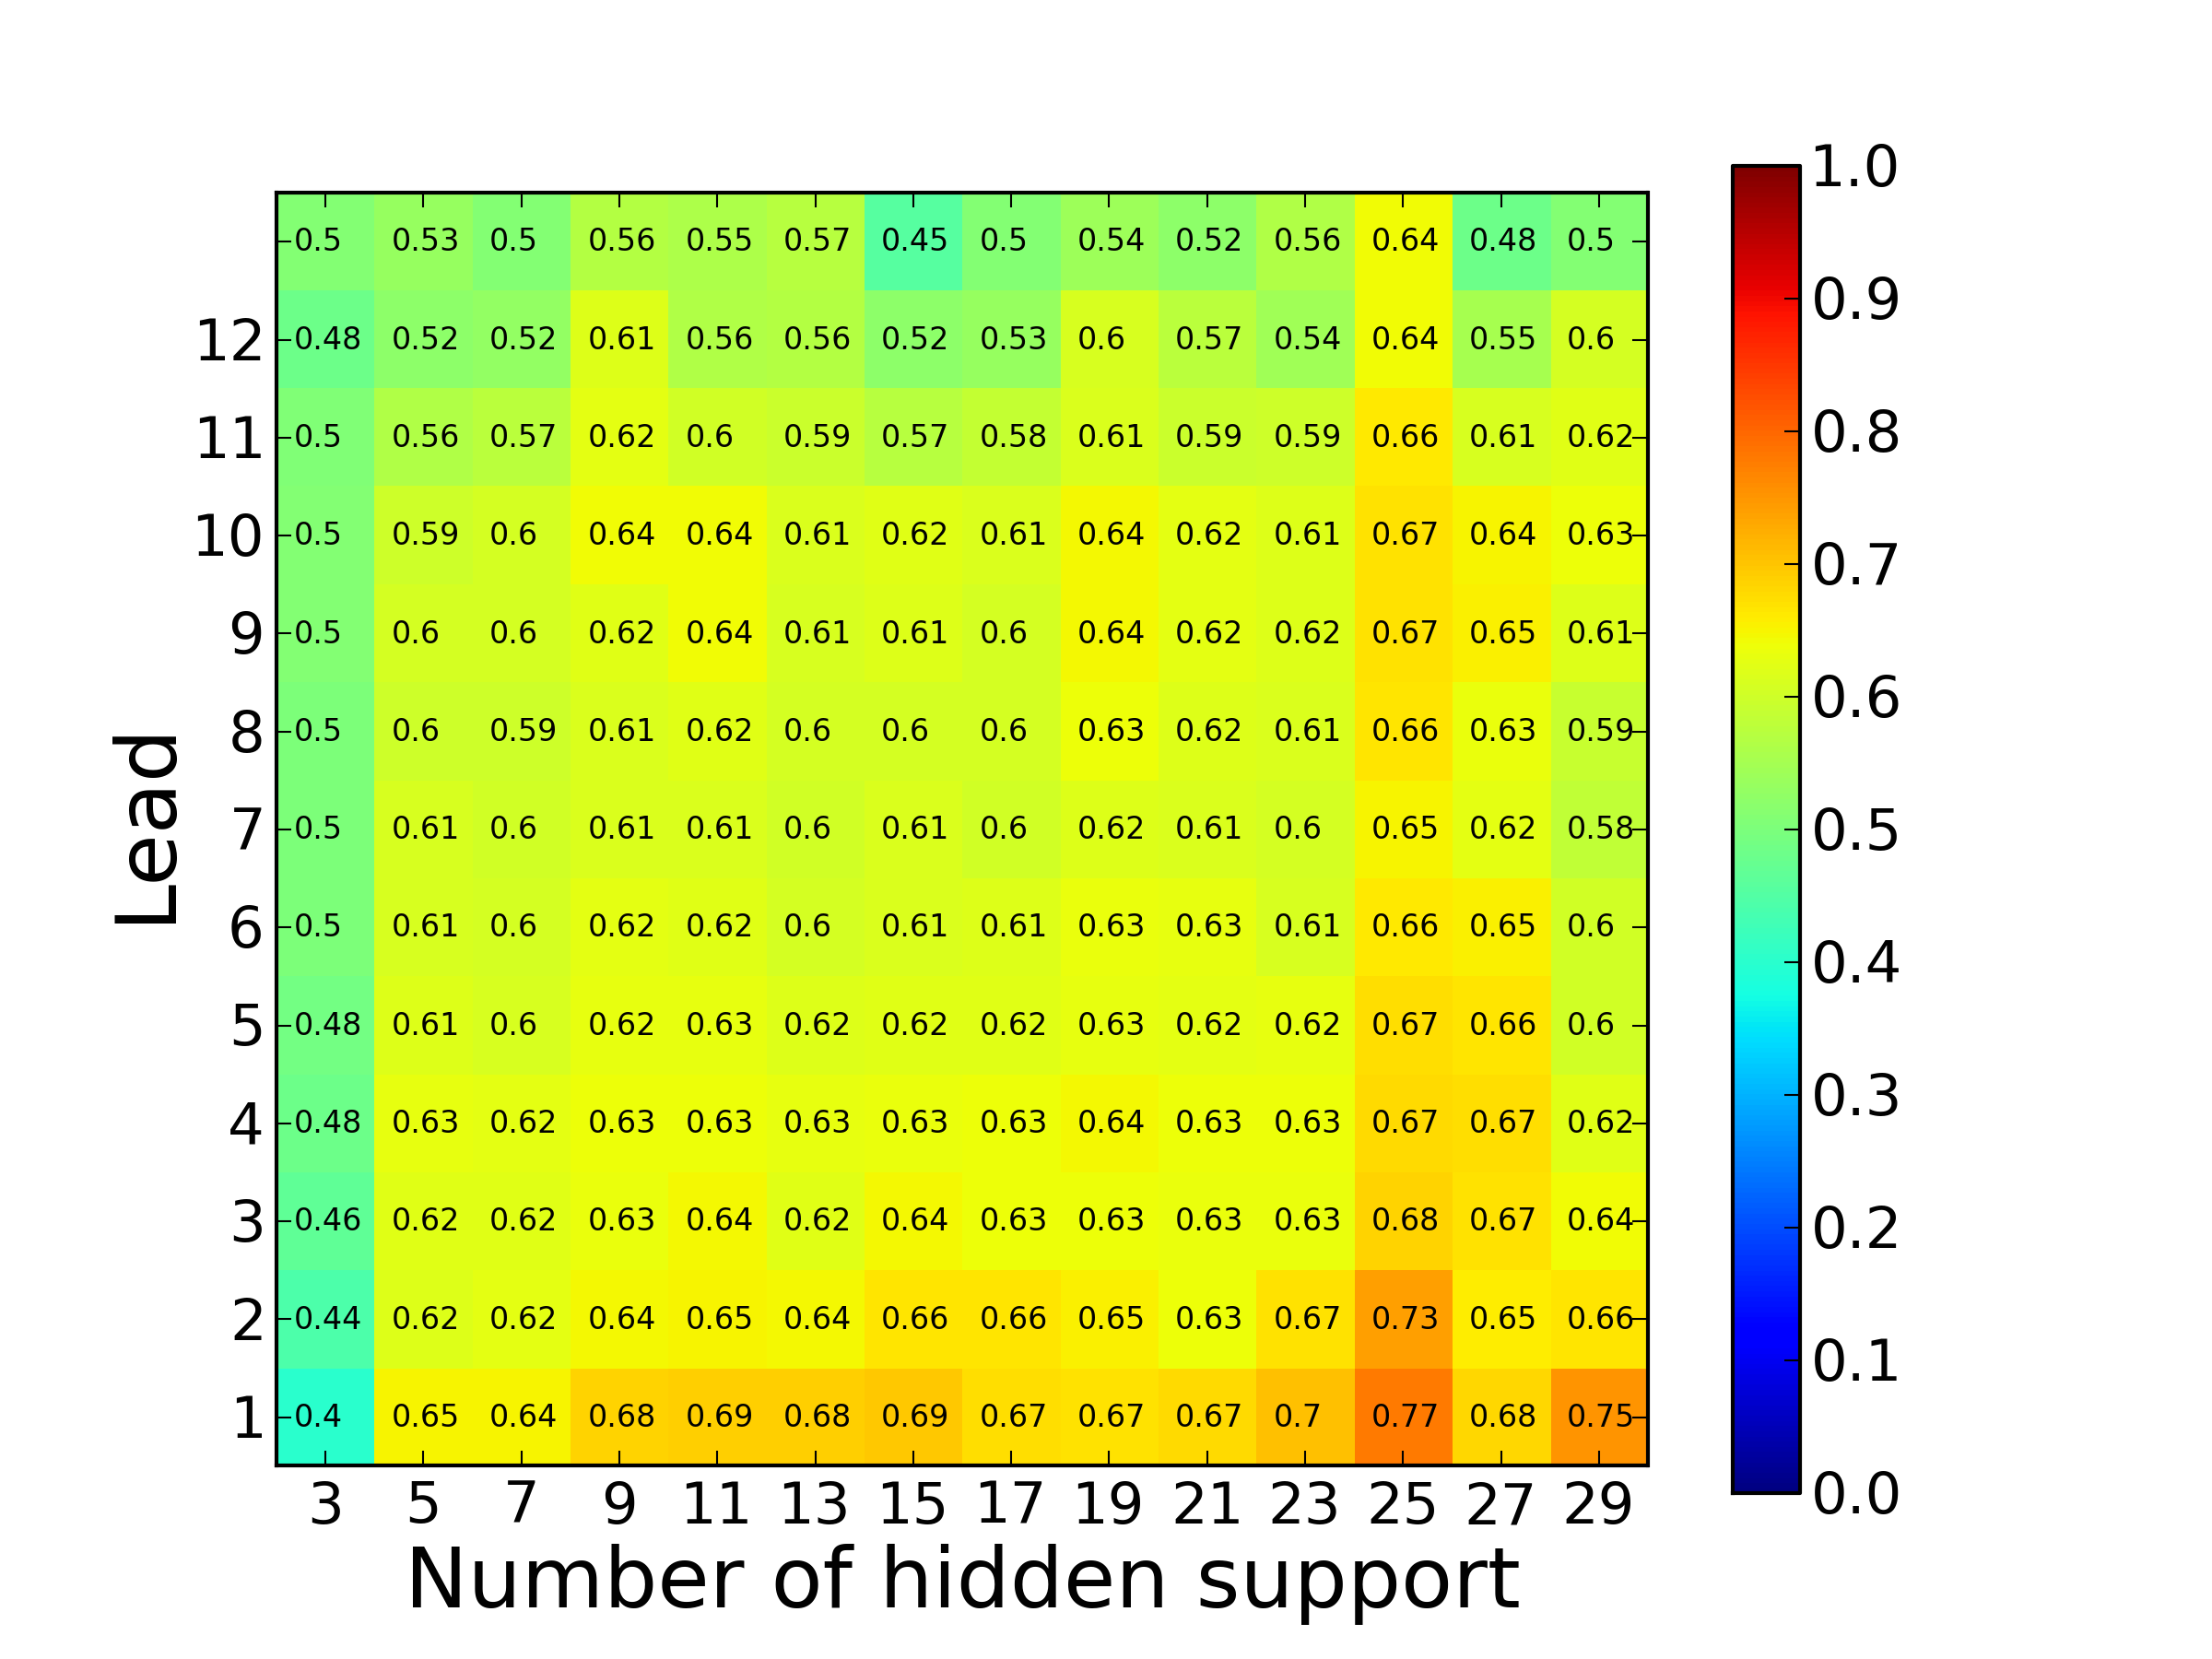
\includegraphics[width=1.0\textwidth]{figures/hmm/wiki_only.png}
\end{figure}

Figures \ref{fig:hmm_heatmap_no_collab} to \ref{fig:hmm_heatmap_wiki_only} show HMM heatmaps for all four cohorts using features that did not undergo principal component analysis. Interestingly, they achieved much different results than the HMMs with PCA. For example, Figure \ref{fig:hmm_heatmap_no_collab} performs consistently better than its PCA counterpart. It converges more quickly- achieving near optimal predictive power at K = 11. It outperforms PCA in nearly every experiment (given K greater than 9), and even attains an AUC of 0.9. This provides further evidence that the PCA HMM did not converge, and it could achieve results as good with a higher K.

However, for other cohorts, such as \forum, the PCA HMM \ref{fig:hmm_heatmap_forum_only} consistently out-predicts the HMM without PCA. The PCA HMM achieves an AUC of ~.78 for all K greater than 19 and lead of one, whereas its non-PCA HMM only hits ~0.82. Similar differences exist in the \both cohort in \ref{fig:hmm_heatmap_forum_and_wiki}. In both of these cohorts, it appears that the PCA HMM used a high enough K to converge to the correct number of modes of students.

One last difference between the non-PCA HMMs and the PCA HMMs is that the non-PCA model's predictive power degrades more gracefully as the lead increases. This remains to be explained and requires more investigation.

\begin{figure}[ht!]
  \caption{Mean AUC as K increases for the \neither cohort.}\label{fig:hmm_support_over_time_no_collab}
  \centering
    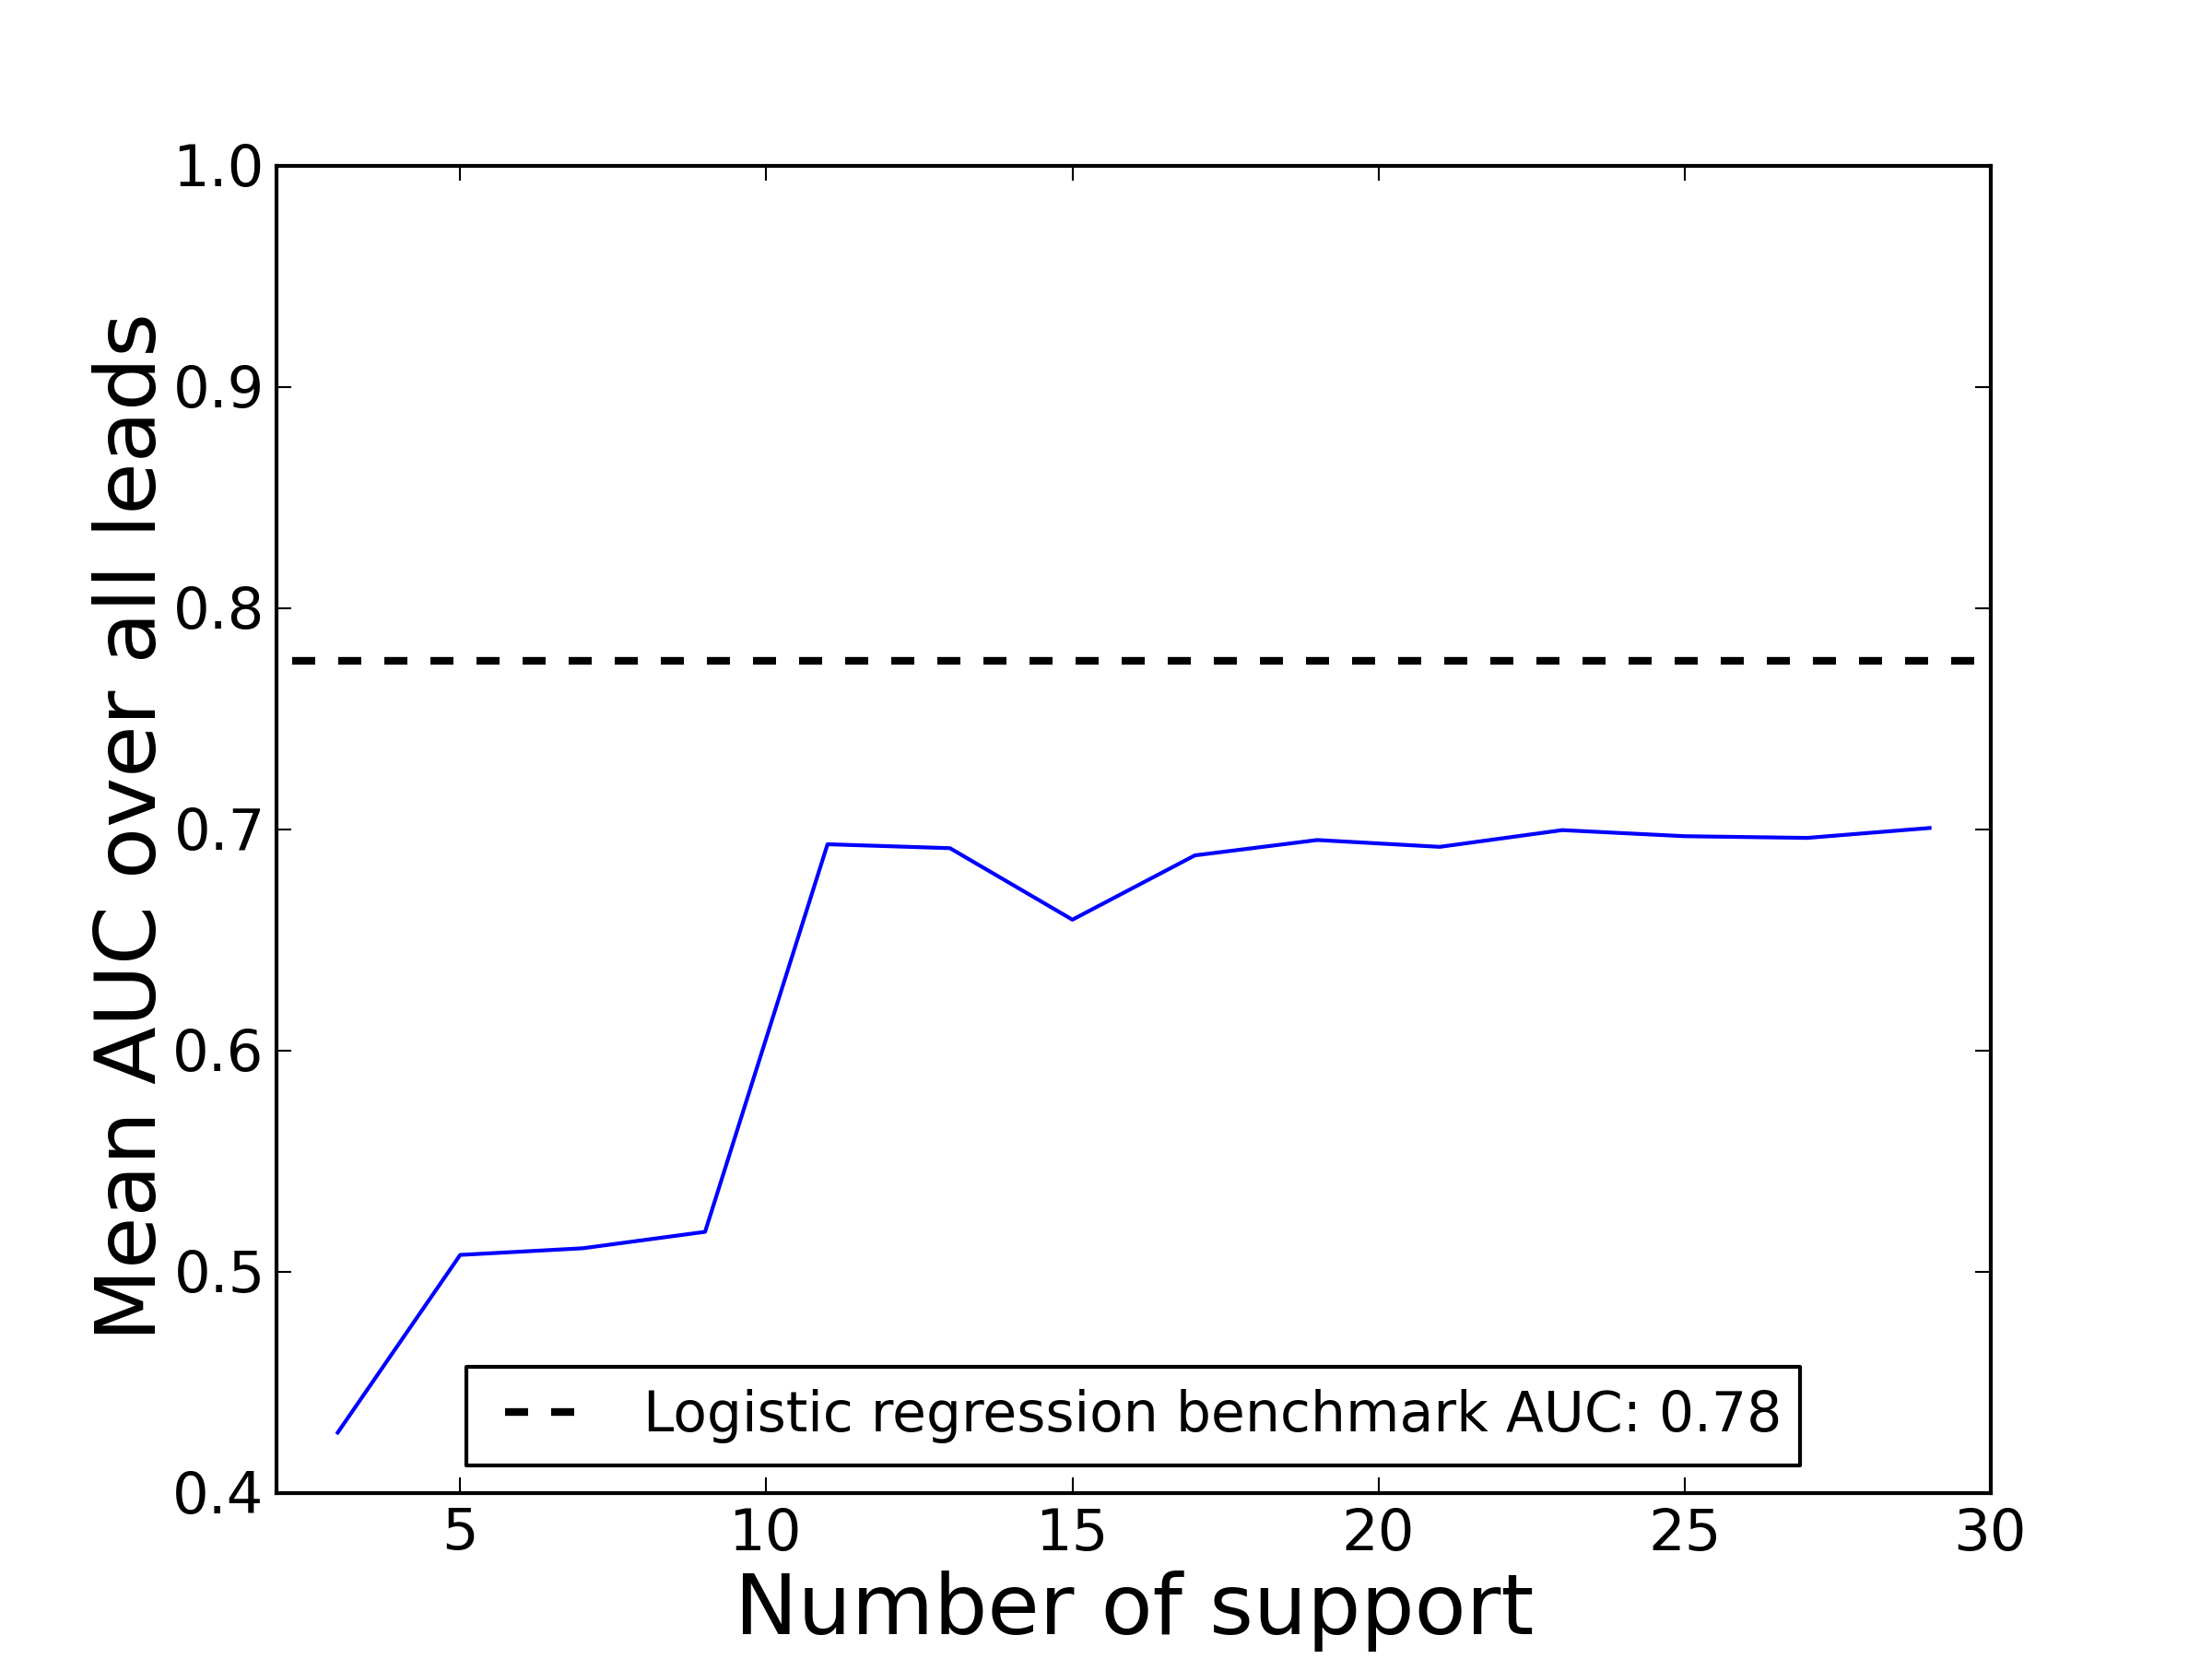
\includegraphics[width=0.8\textwidth]{figures/hmm/no_collab_support_over_time.png}
\end{figure}

\begin{figure}[ht!]
  \caption{Mean AUC as K increases for the \forum cohort.}\label{fig:hmm_support_over_time_forum_only}
  \centering
    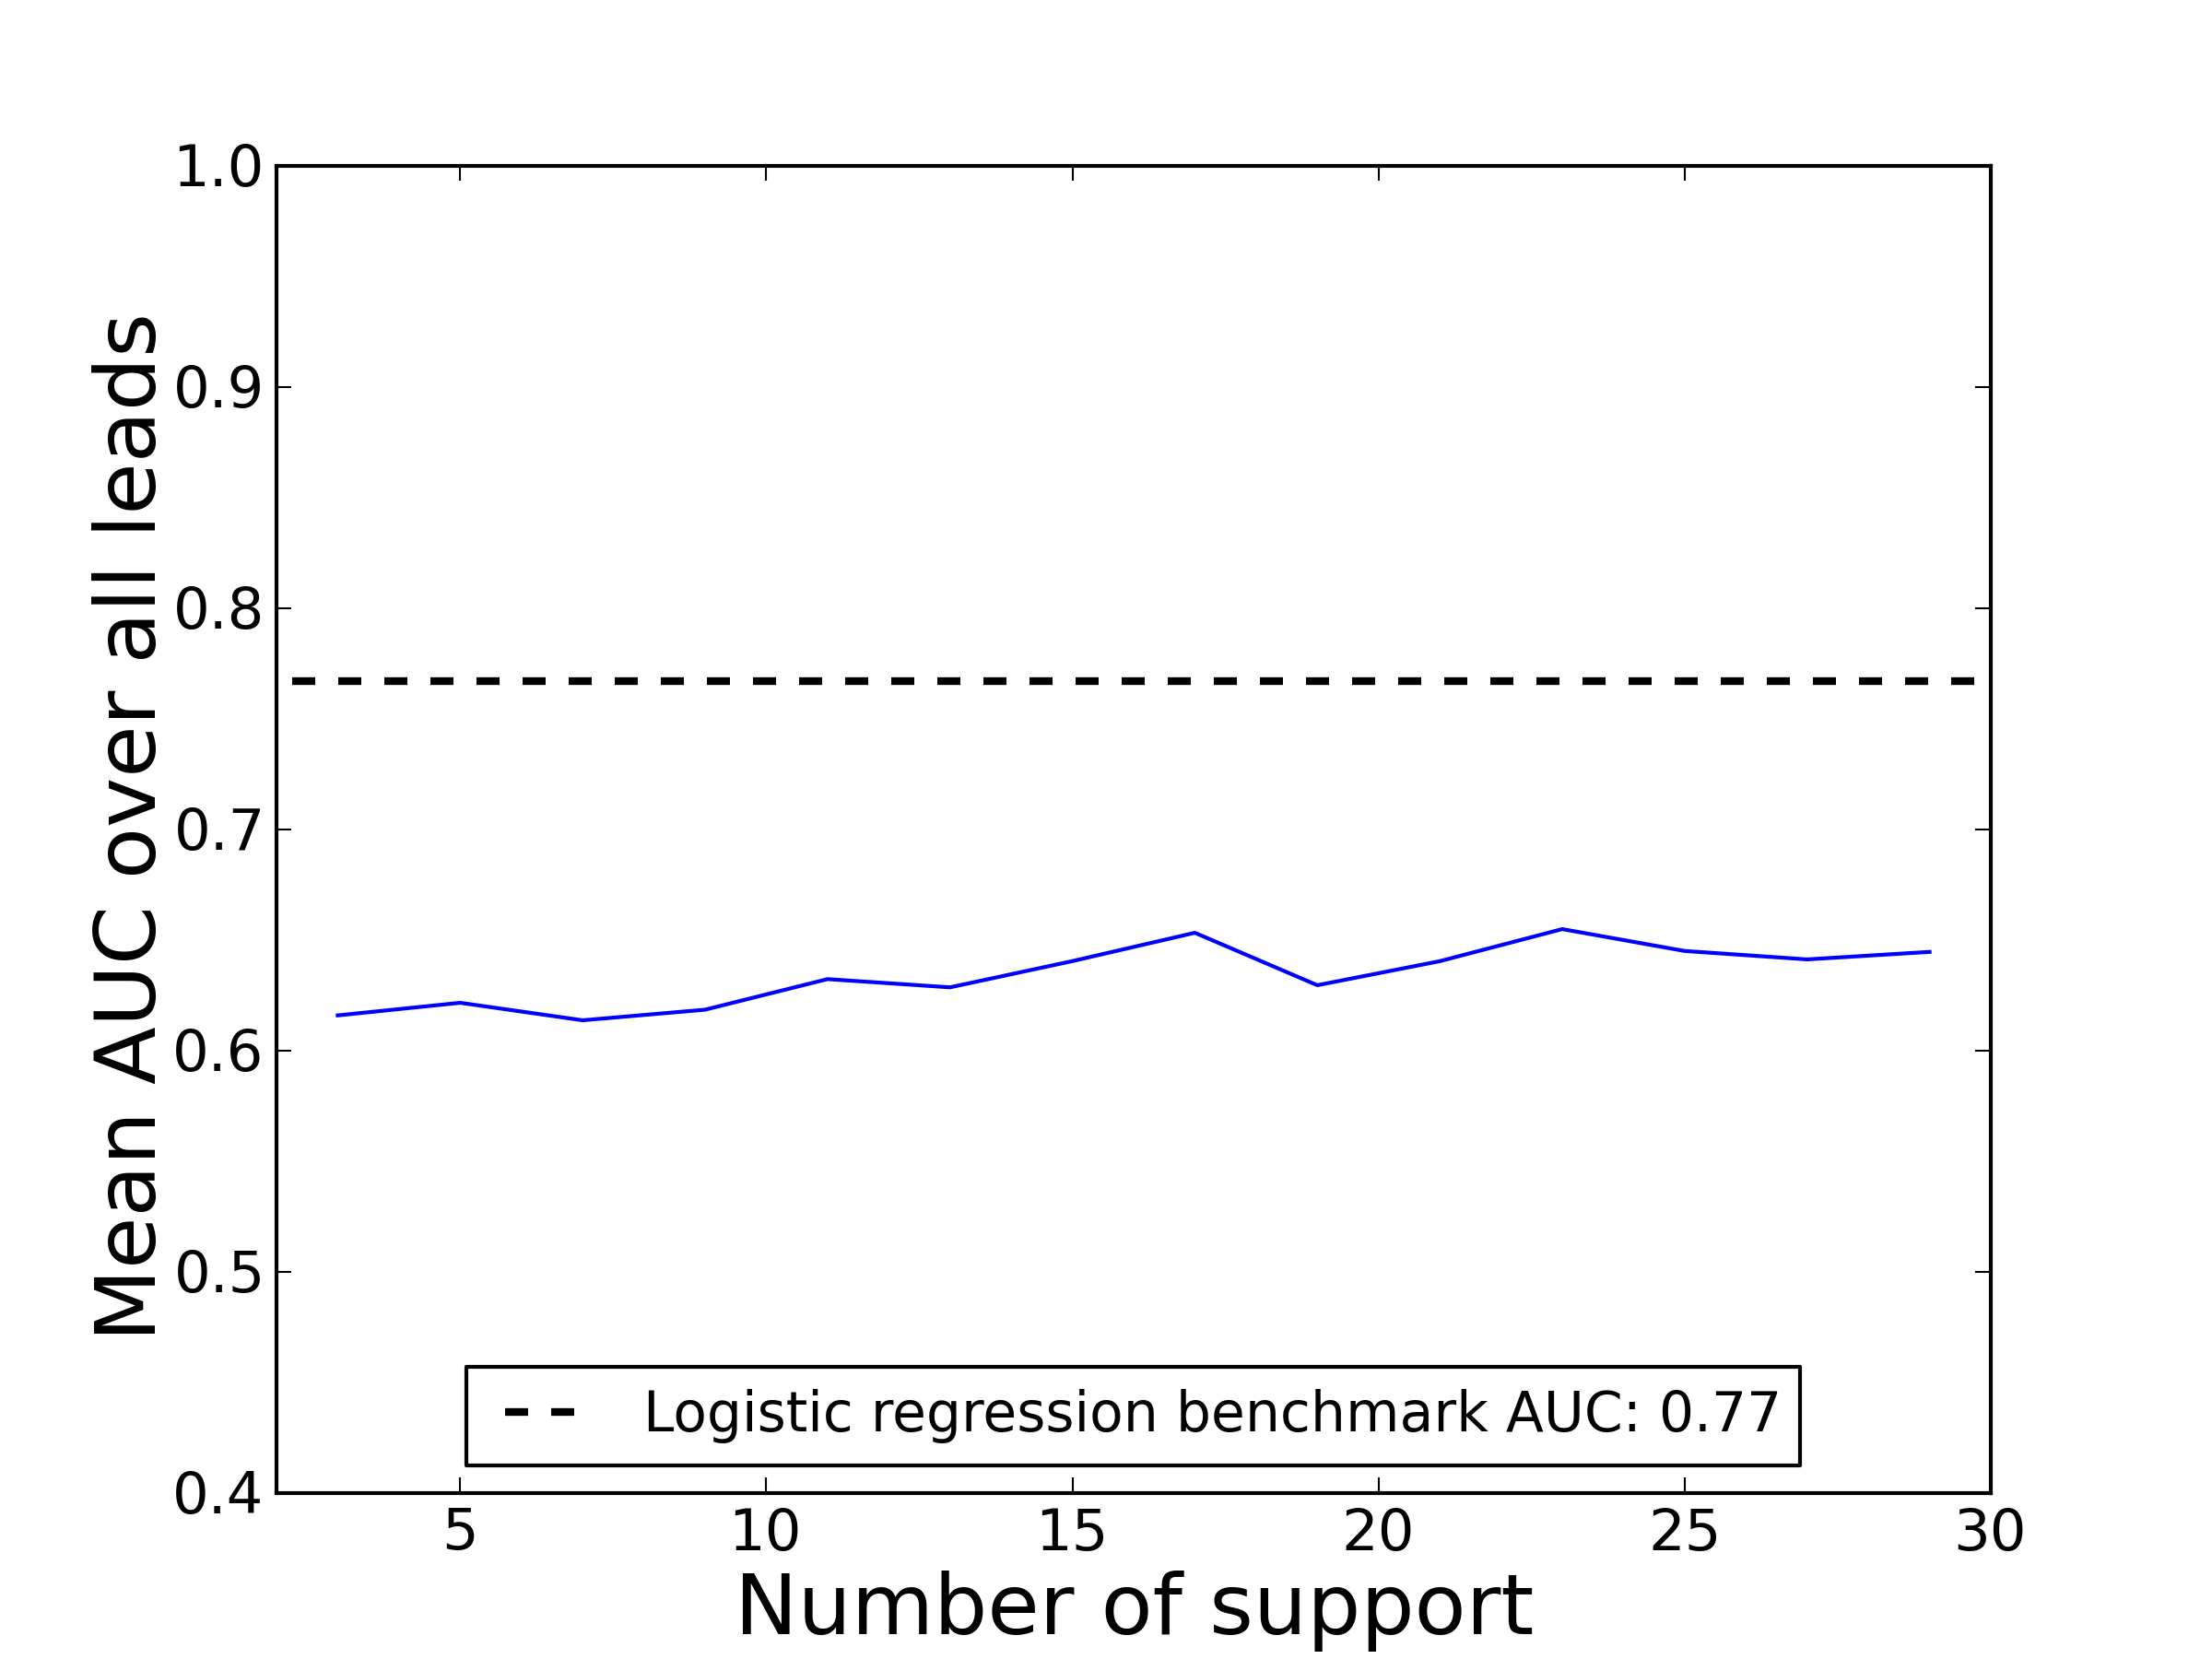
\includegraphics[width=0.8\textwidth]{figures/hmm/forum_only_support_over_time.png}
\end{figure}

\begin{figure}[ht!]
  \caption{Mean AUC as K increases for the \both cohort.}\label{fig:hmm_support_over_time_forum_and_wiki}
  \centering
    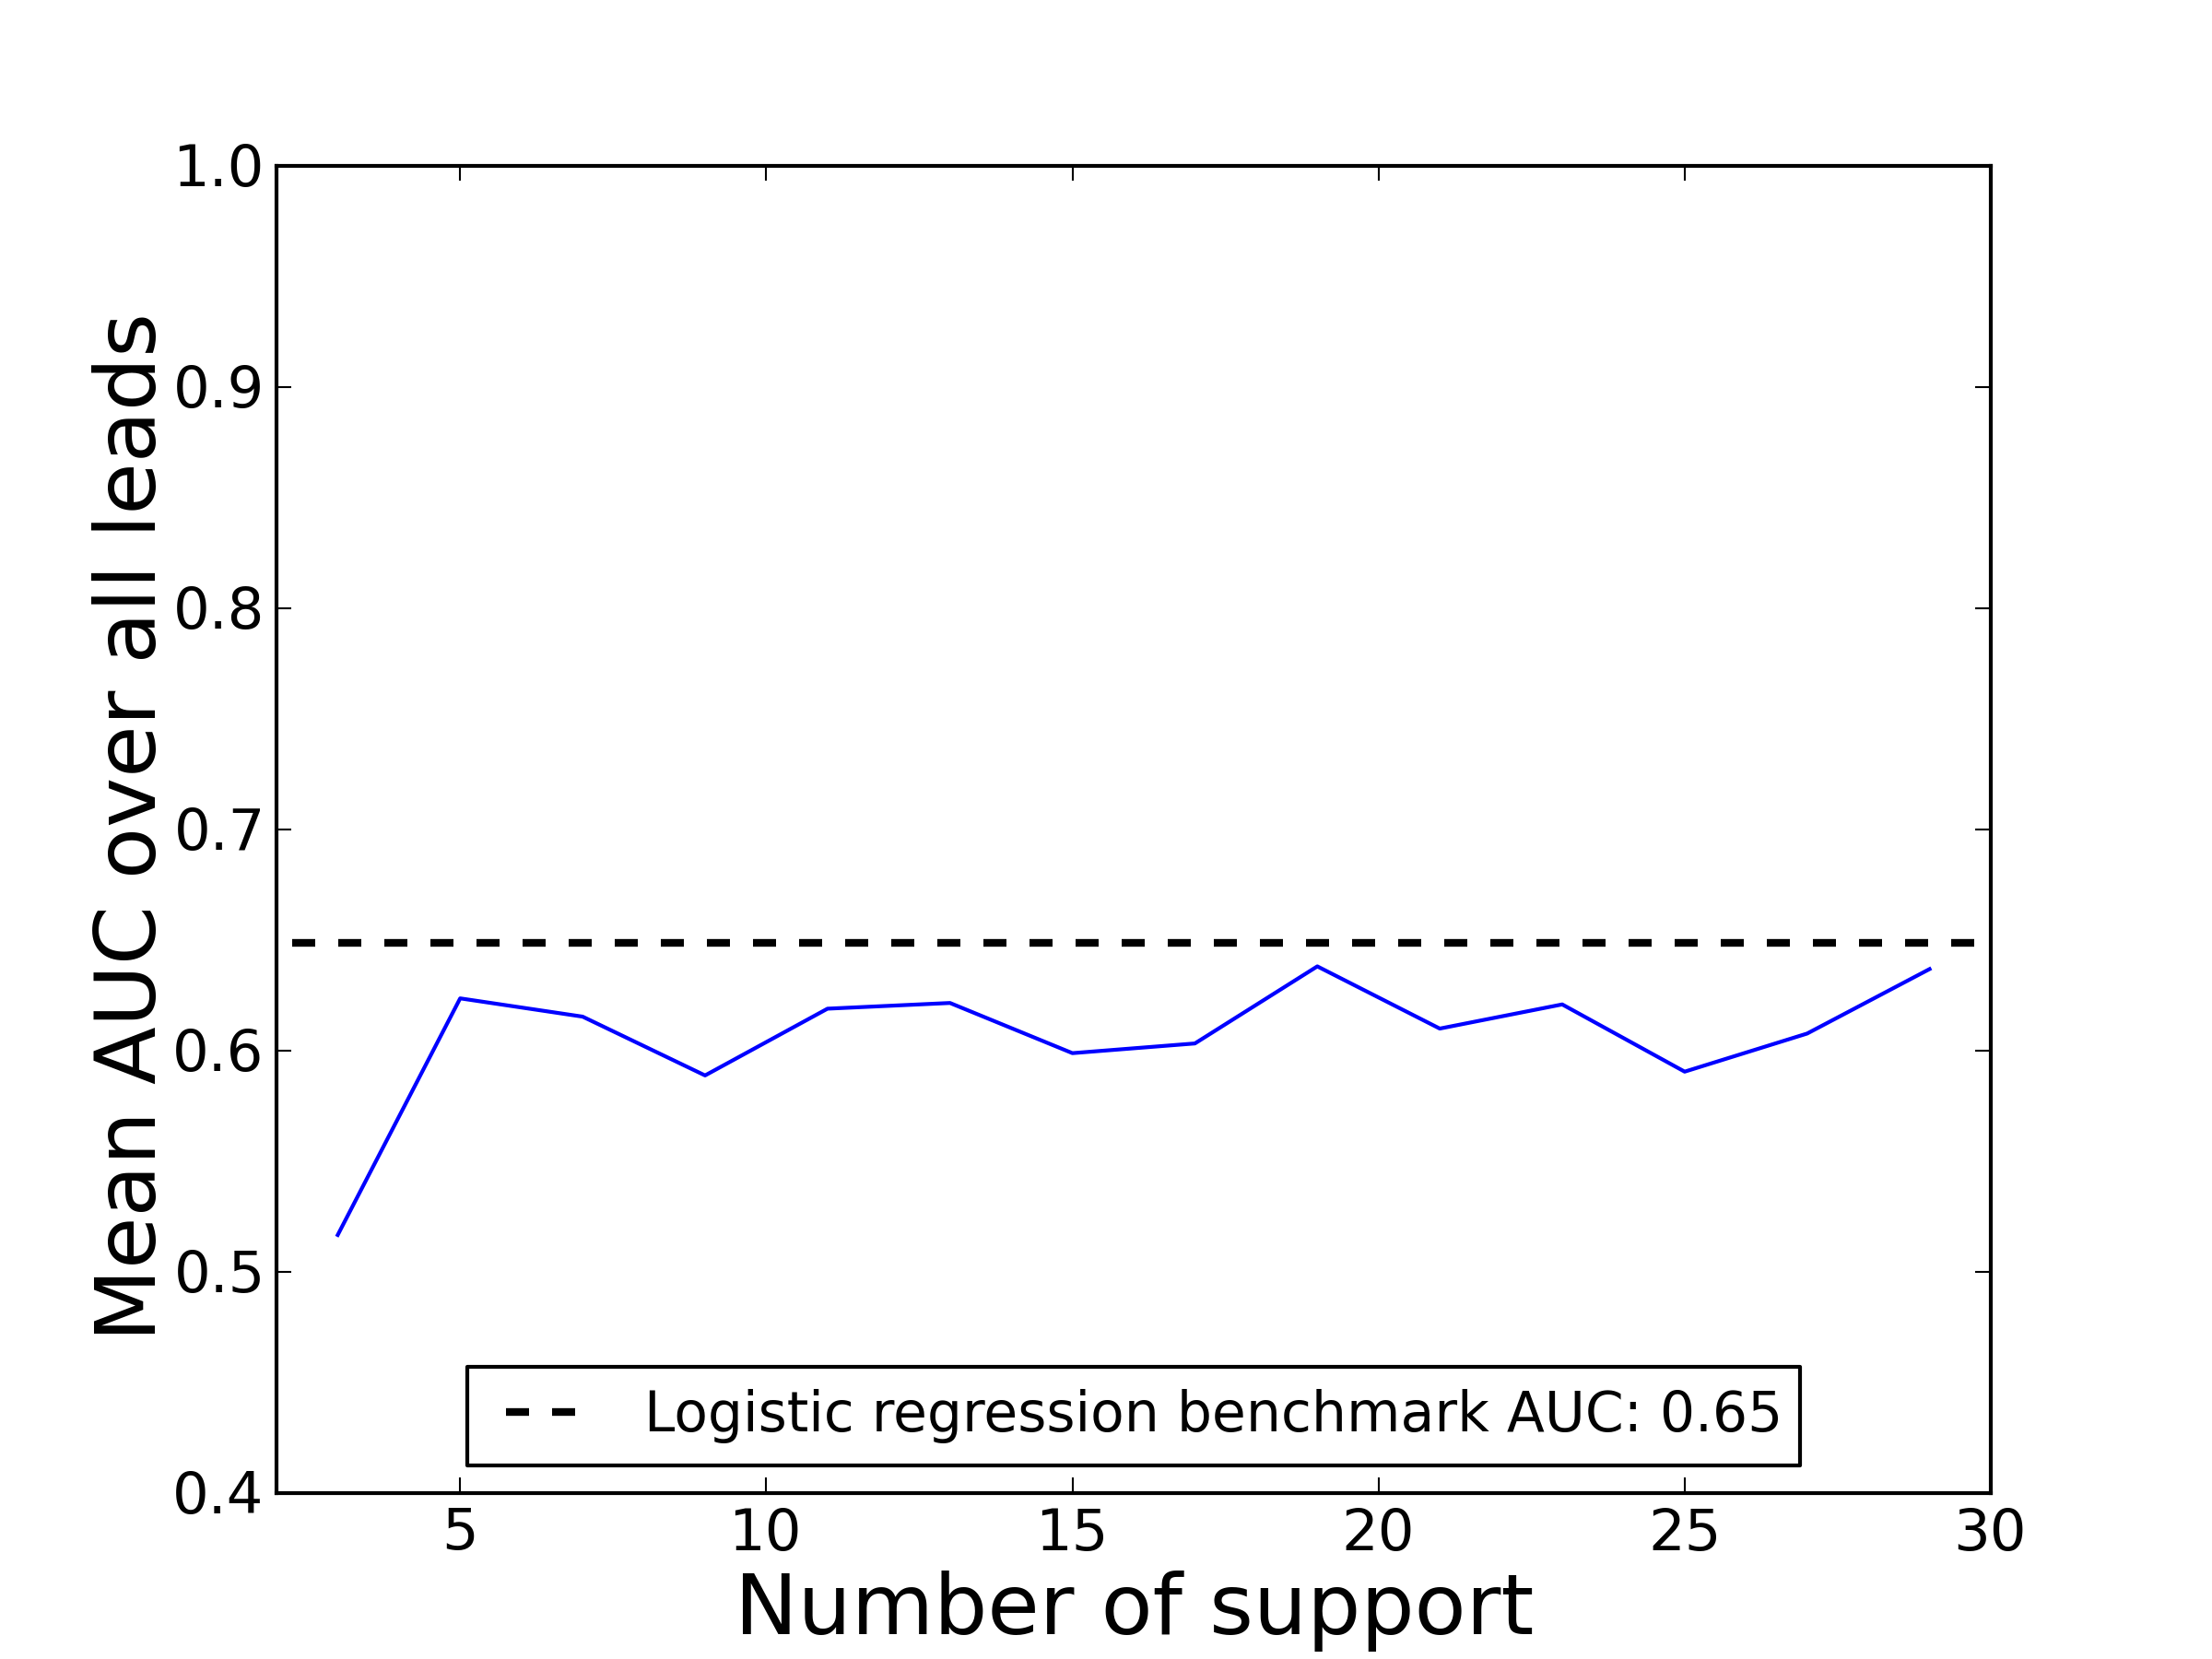
\includegraphics[width=0.8\textwidth]{figures/hmm/forum_and_wiki_support_over_time.png}
\end{figure}

\begin{figure}[ht!]
  \caption{Mean AUC as K increases for the \wiki cohort.}\label{fig:hmm_support_over_time_wiki_only}
  \centering
    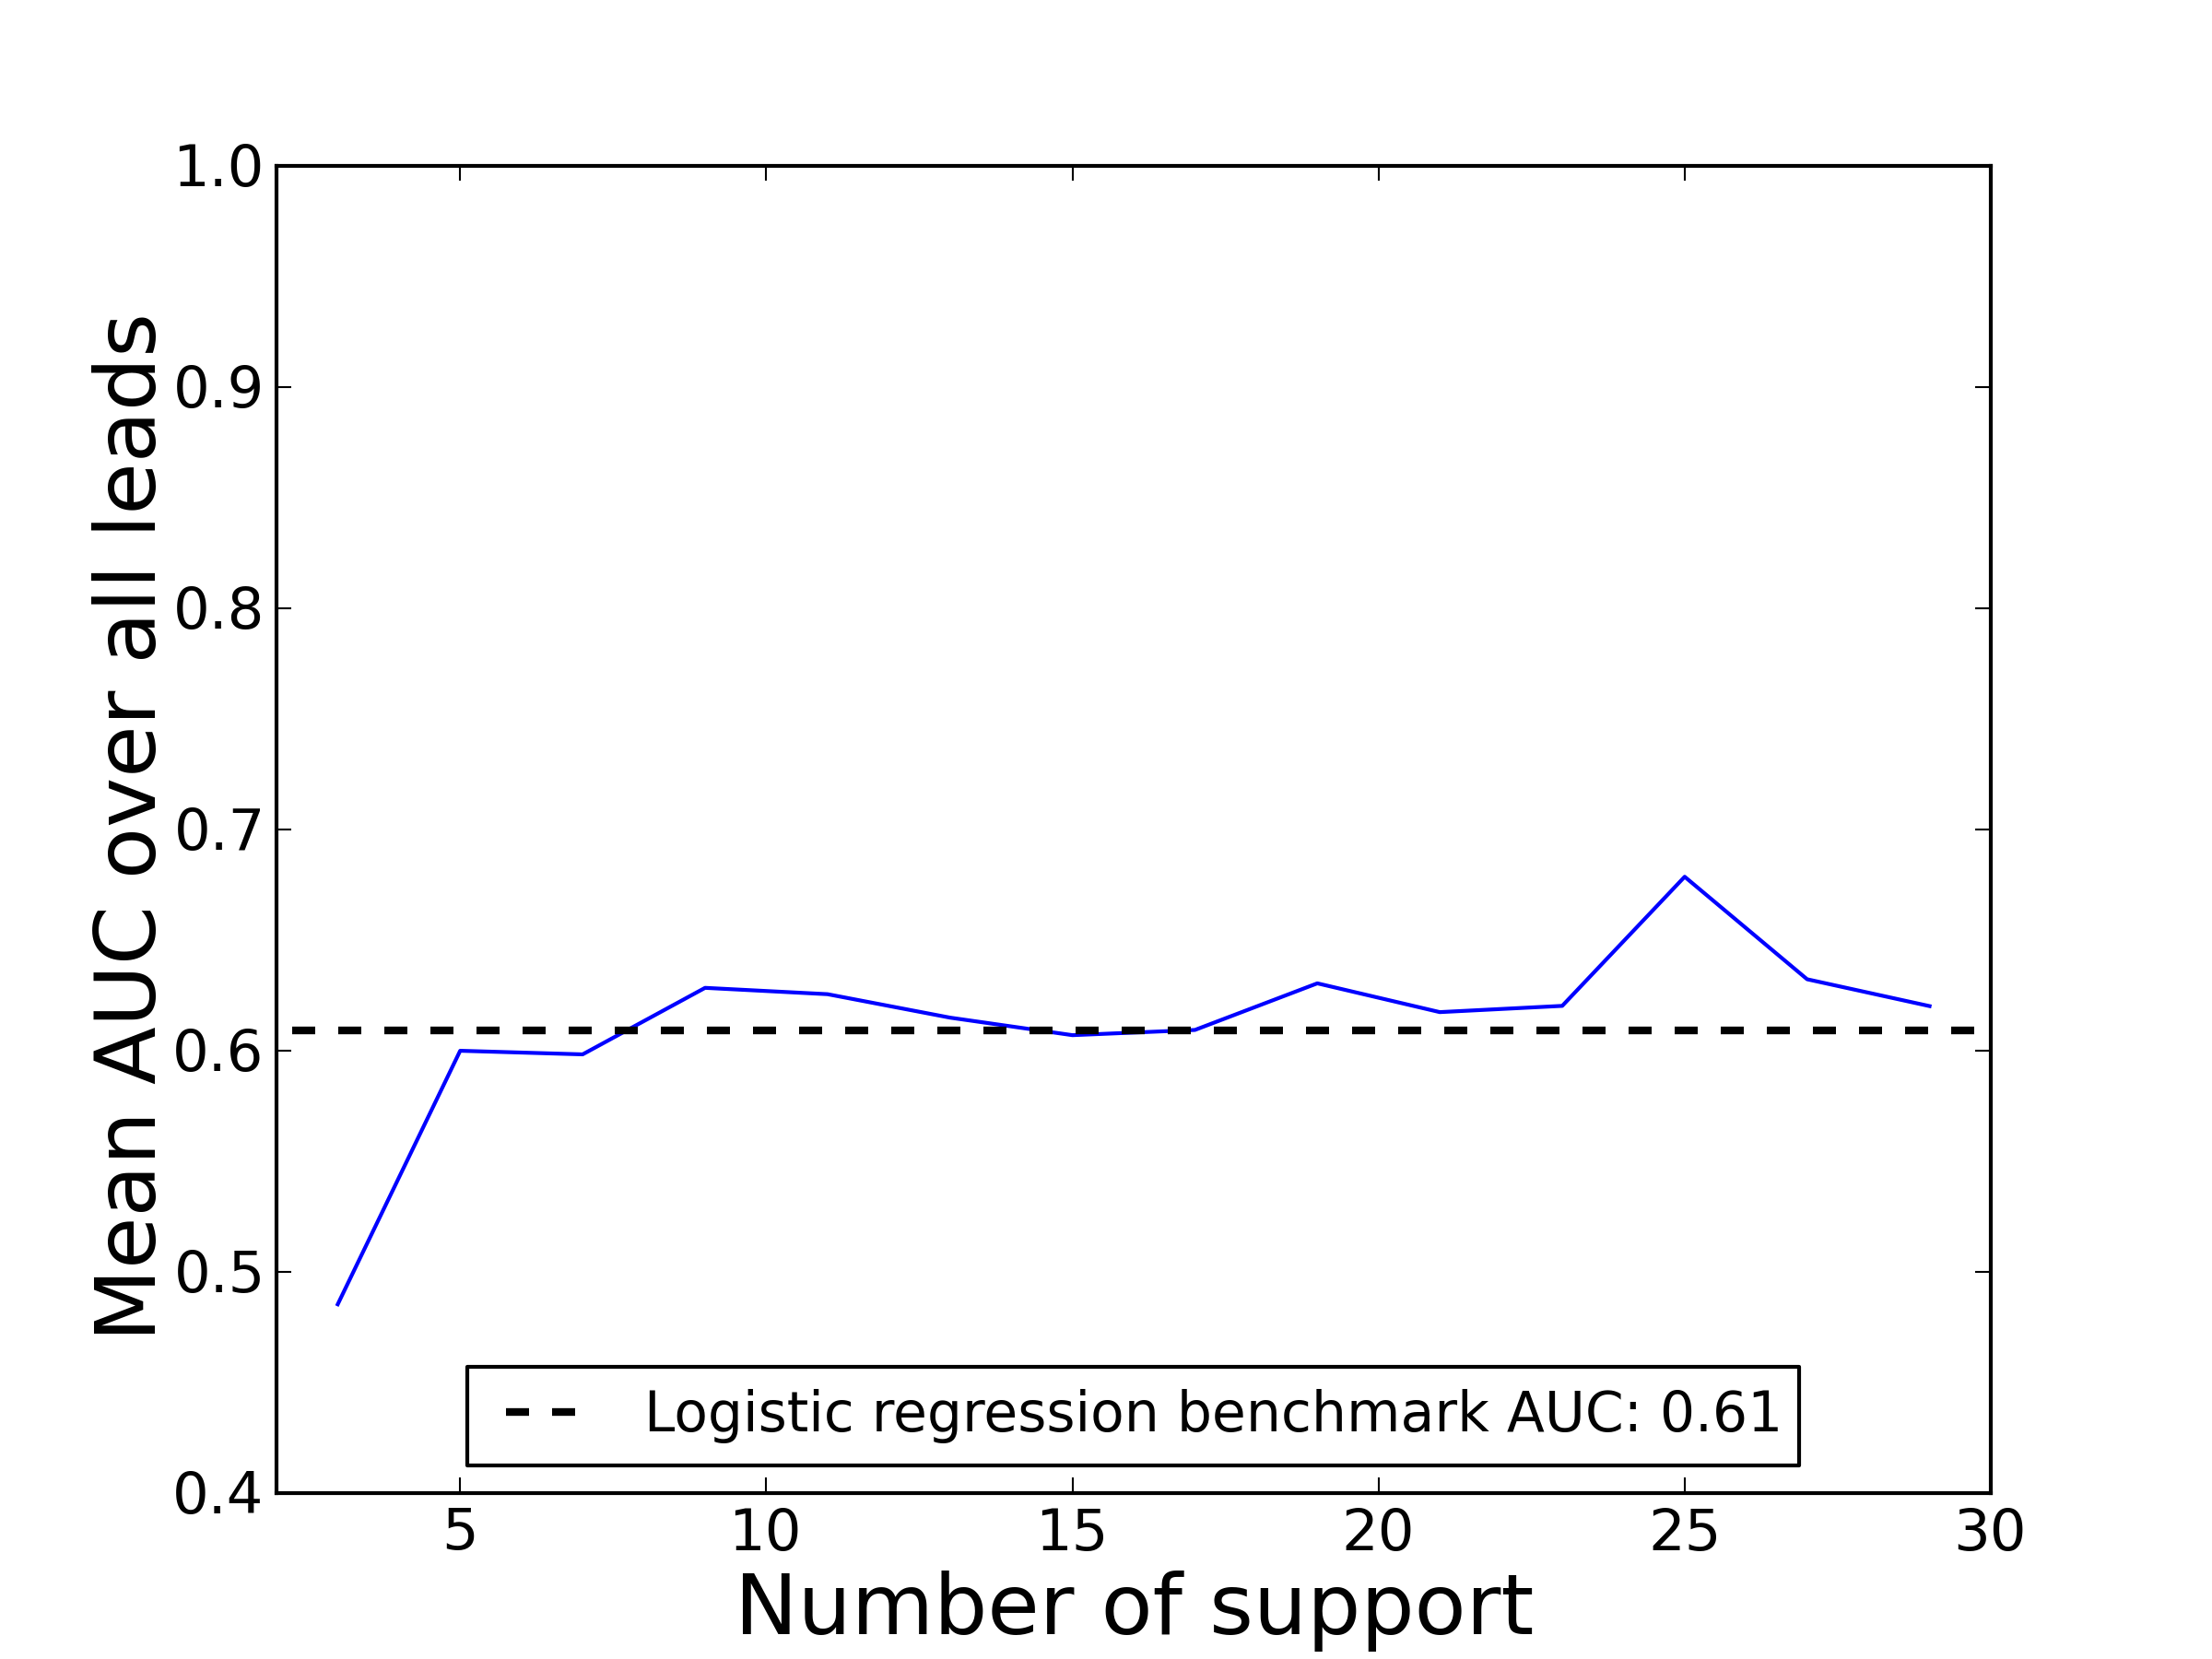
\includegraphics[width=0.8\textwidth]{figures/hmm/wiki_only_support_over_time.png}
\end{figure}

In figures \ref{fig:hmm_support_over_time_no_collab} through \ref{fig:hmm_support_over_time_wiki_only} we look at how the mean AUC changes as K increases for the non-PCA HMMs. We see the AUCs converge much faster than the PCA HMMs. In addition, the mean AUC comes closer to the benchmark logistic regression mean AUC. This is especially true for the smaller \wiki and \both cohorts, on which logistic regression performs poorly due to a lack of data. Indeed, the \wiki HMM outperforms its logistic regression counterpart for almost all values of K.

At this point in the thesis, Chapter \ref{chap:logreg} has described models with logistic regression and Chapter \ref{chap:hmm} with HMMs. HMMs rarely generated AUC results better than logistic regression and were more predictively accurate when we used features not reduced by PCA. Perhaps the best value derived from HMMs is the insight into a hidden state and its support. In Chapter \ref{chap:logreg_hmm} attempt to leverage the hidden state unmasked by HMMs can be used with logistic regression modelling to further extend prediction.
